\chapter{Revisão de Bibliográfica}
	\label{ch:revisao}
	\par Para desenvolver o trabalho, é necessário definir os conceitos de \textit{downsampling}, filtros digitais \textit{wavelets} e energia, que serão usados para a extração de características dos sinais. No processamento dos sinais de voz, serão revisadas as frequências fundamentais da voz, além das escalas BARK e MEL. Também será revisada a engenharia paraconsistente de características, método utilizado para verificar a qualidade das características extraídas. Em seguida, serão estudadas as Interfaces Humano-Máquina para Eletroencefalograma, que coletarão dados das regiões do cérebro. Concluída essa etapa, serão revisadas as Redes Neurais de Pulso, Autoencoders e Redes Neurais Residuais.

	\section{Conceitos utilizados}
		\subsection{Sinais digitais e sub-amostragem (\textit{downsampling})}
			\par Os sinais digitais, tanto de voz quanto aqueles vindos das medições de Eletroencefalograma (ECG), isto é, aqueles que estão amostrados e quantizados \cite{haykin2011sistemas}, constituem a base deste trabalho. Além do processo de digitalização, inerente ao ato de armazenar sinais em computadores, os mesmos podem sofrer, a depender da necessidade ou possibilidade, sub-amostragens ou \textit{downsamplings} \cite{robi2003}. Isso implica em uma estratégia de redução de dimensão e, comumente, ocorre após a conversão de domínio dos sinais com base em filtros digitais do tipo \textit{wavelet}, a serem apresentados adiante. Um exemplo consta na  \autoref{fig:downsampling}, na qual as partes pretas contêm dados e as brancas representam os elementos removidos. Tendo em vista que este trabalho está baseado em sinais digitais de voz e ECG com base em \textit{wavelets}, o processo de sub-amostragem é essencial. 
			\begin{figure}[h]
				\centering
				\caption{Sub-amostragem}
				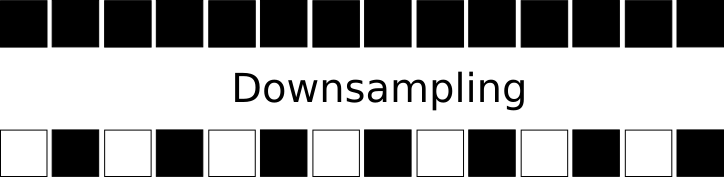
\includegraphics[width=0.4\linewidth]{images/downsampling}
				\label{fig:downsampling}
				\legend{Fonte: O autor}
			\end{figure}
	
		\subsection{Caracterização dos processos de produção da voz humana}
			\par A fala possui três grandes áreas de estudo: A fisiológica, também conhecida como fonética articulatória, a acústica, referida como fonética acústica, e ainda, a perceptual, que cuida da percepção  da  fala \cite{kremer2014eficiencia}. Neste trabalho, o foco será apenas na questão acústica, pois não serão analisados aspectos da fisiologia relacionada à voz, mas sim os sinais sonoros propriamente ditos.
		
		\subsubsection{Sinais vozeados \textit{versus} não-vozeados}
			\par Quando da análise dos sinais de voz, consideram-se as partes vozeadas e não-vozeadas. Aquelas são produzidas com a ajuda da vibração quase periódica das pregas vocais, enquanto estas praticamente não contam com participação regrada da referida estrutura.
		
		\subsubsection{Frequência fundamental da voz}
			\par Também conhecida como $F_0$, é o componente periódico resultante da vibração das pregas vocais. Em termos de percepção, se pode interpretar $F_0$ como o tom da voz, isto é, a frequência de \textit{pitch} \cite{kremer2014eficiencia}. Vozes agudas tem uma frequência de \textit{pitch} alto, enquanto vozes mais graves tem baixa. A alteração da frequência (jitter) e/ou intensidade (shimmer) do \textit{pitch} durante a fala é definida como entonação,  porém, também pode indicar algum distúrbio ou doença relacionada ao trato vocal \cite{WERTZNER2005}.
			
			\par A frequência fundamental da voz é o número de vezes na qual uma forma de onda característica, que reflete a excitação pulmonar moldada pelas pregas vocais, se repete por unidade de tempo. Sendo assim, as medidas de $F_0$ geralmente são apresentadas em Hz \cite{freitas2013avaliaccao}.
			
			\par A medição de $F_0$ está sujeita a contaminações surgidas das variações naturais de \textit{pitch} típicas da voz humana \cite{freitas2013avaliaccao}. A importância de se medir $F_0$ corretamente vem do fato de que, além de carregar boa parte da informação da fala, ela é a base para construção das outras frequências que compõe os sinais de voz, que são múltiplas de $F_0$.
		
		\subsubsection{Formantes}
			\par O sinal de excitação que atravessa as pregas vocais é rico em harmônicas, isto é, frequências múltiplas da fundamental. Tais harmônicas podem ser atenuadas ou amplificadas, em função da estrutura dos tratos vocal e nasal de cada locutor. Particularmente, o primeiro formante ($F_1$), relaciona-se à  amplificação  sonora  na  cavidade  oral  posterior  e  à  posição  da  língua  no  plano  vertical;  o segundo  formante  ($F_2$)  à  cavidade  oral  anterior  e  à  posição  da  língua  no  plano  horizontal; o terceiro  formante  ($F_3$)  relaciona-se  às  cavidades  à  frente  e  atrás  do  ápice  da  língua e, finalmente,  o  quarto formante  ($F_4$) relaciona-se  ao  formato  da  laringe  e  da  faringe  na  mesma  altura  \cite{valencca2014analise}. Formantes caracterizam fortemente os locutores, pois cada indivíduo possui um formato de trato vocal e nasal. Assim, tais frequências, que podem ser capturadas com ferramentas diversas, a exemplo da Transformada \textit{Wavelet}, são de suma importância na área de verificação de locutores.
				
		\subsection{Escalas e energias dos sinais}
			\par A energia de um sinal digital $s[\cdot]$ com $M$ amostras é definida como
			
			\begin{equation}
				E = \sum\limits_{i=0}^{M-1}(s_i)^2 \qquad.   
			\end{equation}
			
			$E$ pode ainda sofrer normalizações e ter a sua mensuração restrita a uma parte específica do sinal sob análise. Possibilidades para tais restrições podem, por exemplo, envolver a escala BARK \cite{doi:10.1121-1.1908630} e MEL \cite{beranek1949acoustic} que serão utilizadas neste trabalho.
		\subsubsection{A escala BARK}
			\par BARK foi definida tendo em mente vários tipos de sinais acústicos. Essa escala corresponde ao conjunto de 25 bandas críticas da audição humana. Suas frequências-base de audiometria são, em Hz: \textbf{20, 100, 200, 300, 400, 510, 630, 770, 920, 1080, 1270, 1480, 1720, 2000, 2320, 2700, 3150, 3700, 4400, 5300, 6400, 7700, 9500, 12000, 15500}. Nessa escala,os sinais digitais no domínio temporal atravessam filtros passa-faixas \cite{bosi2002introduction} para os quais o início e o final da banda de passagem correspondem à frequências-base consecutivas resultando em um vetor de características com 24 coeficientes e, em seguida, as energias dos sinais filtrados são utilizadas como características descritivas de propriedades do sinal sob análise, como mostrado na  \autoref{fig:barkfeaturevect}.
			\begin{figure}[h]
				\centering
				\caption{Cálculo de vetores de características com BARK}
				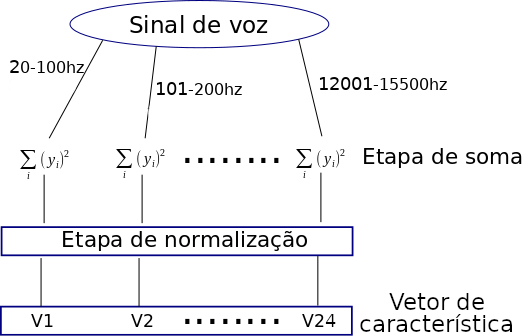
\includegraphics[width=0.6\linewidth]{images/barkFeatureVect}
				\label{fig:barkfeaturevect}
				\legend{Fonte: Elaborado pelo autor}
			\end{figure}
		
		\subsubsection{A escala MEL}
			\par Escala Mel, advinda do termo \textit{melody}, é uma adaptação da escala Bark para sinais de voz. Dentre as várias implementações de bandas críticas a escolhida foi a implementação que contém os valores em Hz: \textbf{20, 160, 394, 670, 1000, 1420, 1900, 2450, 3120, 4000, 5100, 6600, 9000, 14000}.
			
			\par A variante que será usada neste trabalho é conhecida como \textit{Mel-frequency cepstral coefficients}(MFCC) a qual inclui, além dos intervalos definidos, uma diminuição da correlação entre os componentes gerados via aplicação da Transformada Discreta Cosseno (DCT) \cite{salomon2007data} ou da Análise de Componentes Principais (PCA) \cite{jolliffe2006principal} seguida de duas derivações no vetor de características resultando em um total de 11 coeficientes. Nesse trabalho foi escolhida a DCT, no entanto, PCA poderia também ser escolhida sem prejuízos, o uso de uma ou outra depende da preferência do autor.
			
			\par Novamente, desconsiderando qualquer etapa intermediária que possa ser adicionada, as energias calculadas nos intervalos definidos na escala MEL podem, por si mesmas, constituir um vetor de características, como mostrado na  \autoref{fig:barkfeaturevect}.
			
			\begin{figure}[h]
				\centering
				\caption{Cálculo de vetores de características com MEL}
				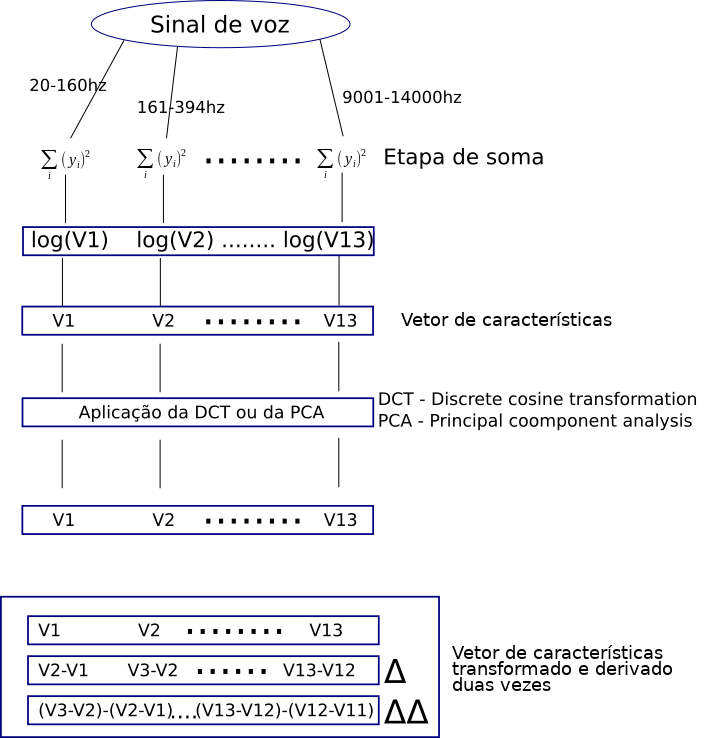
\includegraphics[width=0.6\linewidth]{images/melFeatureVect}
				\label{fig:melfeaturevect}
				\legend{Fonte: Elaborado pelo autor}
			\end{figure}
			
		\subsection{Fala imaginada}
			
			\par A fala imaginada é um fenômeno em que uma pessoa "ouve" a si mesma falando internamente, sem produzir som. As regiões cerebrais usadas na fala imaginada são similares às que estão envolvidas na fala verbal, englobando áreas do córtex motor e pré-motor, além de outras áreas associadas à linguagem e a fala.
			
			\par A ativação cerebral durante processos linguísticos (incluindo a fala imaginada) envolve as seguintes regiões \cite{pinto2012manual}, \cite{Vanderah2020}, \cite{kenhub}:
			
			\begin{itemize}
				\item \textbf{área de Broca}: Localizada no lobo frontal dominante, é crucial para a produção da fala.
				\item \textbf{área de Wernicke}: Situada no lobo temporal e parietal esquerdo, é fundamental para a compreensão da linguagem.
				\item \textbf{córtex motor e pré-motor}: Envolvidos na execução e planejamento dos movimentos necessários para a articulação da fala.
				\item \textbf{giro supramarginal}: Associado à integração sensorial e ao planejamento motor da fala.
				\item \textbf{giro supratemporal e médio}: Responsáveis pelo processamento da compreensão linguística e pela articulação durante a repetição de sílabas.
			\end{itemize}
			
			\par Na maioria dos casos o lobo dominante é o esquerdo, em pessoas canhotas a probabilidade de ser o direito, embora baixa, é maior.
			\par A localização de tais áreas serão mostradas na \autoref{subsec:BCIEEG}.
	
		\subsection{Filtros digitais \textit{wavelet}}
			\par Filtros digitais \textit{wavelet} têm sido utilizados com sucesso para suprir as deficiências de janelamento de sinal apresentadas pelas Transformadas de Fourier e de Fourier de Tempo Reduzido. \textit{Wavelets} contam com variadas funções-filtro e têm tamanho de janela variável, o que permite uma análise multirresolução \cite{Rod5254905}. Particularmente, as \textit{wavelets} proporcionam a análise do sinal de forma detalhada tanto no espectro de baixa frequência quanto no de alta contando com diferentes funções-base não periódicas diferentemente da tradicional transformada de Fourrier que utilizam somente as bases periódicas senoidal e cossenoidal.
			
			\par É importante observar que, quando se trata de Transformadas \textit{Wavelet}, seis elementos estão presentes: dois filtros de análise, dois filtros de síntese e as funções ortogonais \textit{scaling} e \textit{wavelet}. No tocante a sua aplicação, só a transformada direta, e não a inversa, será usada na construção dos vetores de características. Portanto, os filtros de síntese, a função \textit{scaling} e a função \textit{wavelet} não serão elementos abordados aqui: eles somente interessariam caso houvesse a necessidade da transformada inversa.
			
			\par No contexto dos filtros digitais baseados em \textit{wavelets}, o tamanho da janela recebe o nome de \textbf{suporte}. Janelas definem o tamanho do filtro que será aplicado ao sinal. Quando esse é pequeno (limitado), se diz que a janela tem \textbf{um suporte compacto} \cite{robi2003}.
			
			\par Se diz que uma \textit{wavelet} tem boa \textbf{resposta em frequência} quando, na aplicação da mesma para filtragem, não são causadas muitas pertubações indesejadas ao sinal, no domínio da frequência. Os filtros \textit{wavelet} de Daubechies \cite{daubechies1992ten} se destacam nesse quesito por serem \textit{maximamente planos} (\textit{maximally-flat}) \cite{butterworth1930} \cite{bianchi2007electronic} nos platôs de resposta em frequência como indicado na  \autoref{fig:daubechies} ao contrário do que ocorre na  \autoref{fig:nomaximallyflat}.
			
			\begin{figure}[h]
				\centering
				\caption[Platôs maximamente planos Daubechies]{Platôs maximamente planos em um filtro digital: característica da família de Daubechies}
				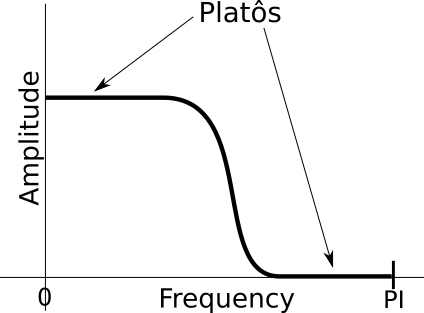
\includegraphics[width=0.3\linewidth]{images/daubechies}
				\label{fig:daubechies}
				\legend{Fonte: Elaborado pelo autor}
			\end{figure}
			
			\begin{figure}[h]
				\centering
				\caption[Platôs maximamente planos outros filtros]{Platôs não maximamente planos de um filtro digital: características de outros filtros \textit{wavelet}, distintos da família de Daubechies}
				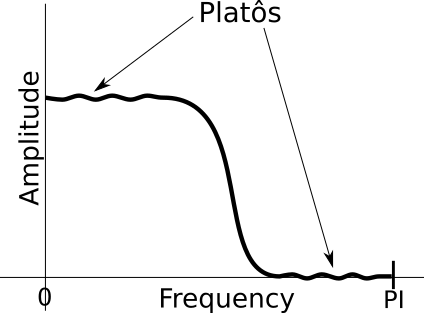
\includegraphics[width=0.3\linewidth]{images/noMaximallyFlat}
				\label{fig:nomaximallyflat}
				\legend{Fonte: Elaborado pelo autor}
			\end{figure}
			
			\par Além da resposta em frequência, na aplicação de um filtro digital \textit{wavelet} também é possível considerar a \textbf{resposta em fase}, que constitui um atraso ou adiantamento do sinal filtrado em relação ao sinal original, ambos no domínio temporal. Esse deslocamento pode ser \textbf{linear}, \textbf{quase linear} ou \textbf{não linear}: 
	
			\begin{itemize}
				\item na resposta em fase \textbf{linear}, há o mesmo deslocamento de fase para todos os componentes do sinal;
				\item quando a resposta em fase é \textbf{quase linear} existe uma pequena diferença no deslocamento dos diferentes componentes do sinal;
				\item finalmente, quando a resposta é \textbf{não linear}, acontece um deslocamento significativamente heterogêneo para as diferentes frequências que compõe o sinal.
			\end{itemize}
			
			\par Idealmente, é desejável que todo filtro apresente boa resposta em frequência e em fase linear. Características de fase e frequência de algumas famílias de filtros \textit{wavelet} constam na Tabela \autoref{tab:waveletsProperties}.
			
			\begin{table}[h]
	\centering
	\caption{Algumas das \textit{wavelets} mais usadas e suas propriedades}
	\begin{tabular}{|c|p{75mm}|c|}
			\hline 
			\textbf{Wavelet} & \textbf{Resposta em frequência} & \textbf{Resposta em fase} \\ 
			\hline 
			Haar & Pobre &  Linear \\ 
			\hline 
			Daubechies & mais próxima da ideal à medida que o \newline  suporte aumenta; \textit{maximally-flat}  &  Não linear \\ 
			\hline 
			Symmlets & mais próxima da ideal à medida que o \newline  suporte aumenta; não \textit{maximally-flat}  & Quase linear \\ 
			\hline 
			Coiflets & mais próxima da ideal à medida que o \newline  suporte aumenta; não \textit{maximally-flat}  & Quase linear \\ 
			\hline 
	\end{tabular} 
	\label{tab:waveletsProperties}
	\\Fonte: Elaborado pelo autor, 2022.
\end{table}

	
		\subsubsection{O algoritmo de Mallat para a Transformada \textit{Wavelet}}
			\par Baseando-se no artigo \cite{7079589}, percebe-se que algoritmo de Mallat faz com que aplicação das \textit{wavelets} seja uma simples multiplicação de matrizes. O sinal que deve ser transformado se torna uma matriz linear vertical. Os filtros passa-baixa e passa-alta tornam-se, nessa ordem, linhas de uma matriz quadrada que será completada segundo regras que serão mostradas mais adiante. É importante que essa matriz quadrada tenha a mesma dimensão que o sinal a ser transformado.
			
			\par Interessantemente, para que seja possível a transformação \textit{wavelet}, basta ter disponível o vetor do filtro passa-baixas calculado a partir da \textit{mother wavelet}, que é a função geradora desse filtro, já que o passa-alta pode ser construído a partindo-se da ortogonalidade do primeiro.
			
			\par Determinar a ortogonal de um vetor significa construir um vetor, tal que, o produto escalar do vetor original com sua respectiva ortogonal seja nulo.
			
			\par Considerando $h[\cdot]$ como sendo o vetor do filtro passa-baixas e $g[\cdot]$ seu correspondente ortogonal, tem-se que $h[\cdot] \cdot g[\cdot] = 0 \qquad .$
			\par Portanto, se $h[\cdot]=[a, b, c, d]$ então seu ortogonal será $g[\cdot]=[d, -c, b, -a]$ pois:
			$$
			h[\cdot] \cdot g[\cdot]  =  [a, b, c, d] \cdot [d, -c, b, -a] = (a \cdot d) + (b \cdot (-c)) + (c \cdot b) + (d \cdot (-a)) = ad - ad + bc - bc = 0 \qquad.
			$$
	
			\par A título de exemplo, considera-se:
			\begin{itemize}
				\item o filtro passa baixa baseado na \textit{wavelet} Haar: $h[\cdot] = [\frac{1}{\sqrt{2}}, \frac{1}{\sqrt{2}}]$
				\item o seu respectivo vetor ortogonal: $g[\cdot] = [\frac{1}{\sqrt{2}}, \frac{-1}{\sqrt{2}}]$
				\item e também o seguinte sinal-exemplo de entrada: $s = \{1,2,3,4\}$
			\end{itemize}
			
			\par Se o tamanho do sinal a ser tratado é quatro e se pretende-se aplicar o filtro Haar, a seguinte matriz de coeficientes é construída:
			\begin{equation}
				\begin{pmatrix}
					\frac{1}{\sqrt{2}}, \frac{1}{\sqrt{2}}, 0, 0\\
					\frac{1}{\sqrt{2}}, \frac{-1}{\sqrt{2}}, 0, 0\\
					0, 0, \frac{1}{\sqrt{2}}, \frac{1}{\sqrt{2}}\\
					0, 0, \frac{1}{\sqrt{2}}, \frac{1}{\sqrt{2}}
					\label{eq:haarFilters}
				\end{pmatrix} 
			\end{equation}
		
			\par Tendo em vista que a dimensão do sinal sob análise é diferente da dimensão do filtro, basta completar cada uma das linhas da matriz de coeficientes com zeros. A matriz é montada de forma que ela seja ortogonal.
			
			\par Montada a matriz de filtros, segue-se com os cálculos da transformada:
			\begin{equation}
				\begin{pmatrix}
					\frac{1}{\sqrt{2}}, \frac{1}{\sqrt{2}}, 0, 0\\
					\frac{1}{\sqrt{2}}, \frac{-1}{\sqrt{2}}, 0, 0\\
					0, 0, \frac{1}{\sqrt{2}}, \frac{1}{\sqrt{2}}\\
					0, 0, \frac{1}{\sqrt{2}}, \frac{1}{\sqrt{2}}\\
				\end{pmatrix} 
				\cdot
				\begin{pmatrix}
					1\\
					2\\
					3\\
					4\\
				\end{pmatrix} 
				=
				\begin{pmatrix}
					\frac{3}{\sqrt{2}}\\
					\frac{-1}{\sqrt{2}}\\
					\frac{7}{\sqrt{2}}\\
					\frac{-1}{\sqrt{2}}
				\end{pmatrix}
				\label{eq:haarMultiplic}
			\end{equation}

			\par Realizada a multiplicação, é necessário montar o sinal filtrado. Isso é feito escolhendo, dentro do resultado, valores alternadamente de forma que o vetor resultante seja:
			
			\begin{equation}
				resultado = \Big[
				\frac{3}{\sqrt{2}},
				\frac{7}{\sqrt{2}},
				\frac{-1}{\sqrt{2}},
				\frac{-1}{\sqrt{2}}
				\Big]\qquad.
				\label{eq:haarResult}
			\end{equation}
			
			\par Percebe-se que, na transformação descrita nas Equações \autoref{eq:haarFilters}, \autoref{eq:haarMultiplic} e \autoref{eq:haarResult}, a \textbf{aplicação dos filtros sobre o vetor de entrada ocorreu apenas uma vez}. Sendo assim, se diz que o sinal recebeu uma \textbf{transformação de nível 1}. A cada transformação, há uma separação do sinal em dois componentes: o de baixa e o de alta frequência.
	
			\par Embora haja um limite, que será mencionado adiante, é possível aplicar mais de um nível de decomposição ao sinal. Para que se possa fazer isso, a Transformada \textit{Wavelet} nível 2 deve considerar apenas a parte de baixas frequências da primeira transformada; a transformada de nível 3 deve considerar apenas a parte de baixas frequências da transformada nível 2, e assim consecutivamente.
			
			\par Nos exemplos numéricos mostrados nas Tabelas \autoref{tab:regularWaveletExample}, \autoref{tab:packetWaveletExampleLF} e \autoref{tab:packetWaveletExampleHF}, usou-se um filtro normalizado cujos coeficientes são $\{\dfrac{1}{2},-\dfrac{1}{2}\}$. Os dados destacados em \textbf{verde} correspondem ao \textbf{vetor original} que será tratado. Cada uma das linhas são os resultados das transformações nos níveis 1, 2, 3 e 4, respectivamente. As partes em \textbf{azul} correspondem à porção de \textbf{baixas frequências}, enquanto que as partes em \textbf{amarelo} correspondem às porções de \textbf{altas frequências}.
			
			\par Percebe-se que na Tabela \autoref{tab:regularWaveletExample}, a partir da transformação nível 2, apenas as partes de baixa frequência são modificadas. Isso implica que, no momento da implementação do algoritmo de Mallat \textbf{para níveis maiores que 1}, a abordagem será \textbf{recursiva}. Em outras palavras, a partir do nível 1 se deve aplicar Mallat apenas às porções de baixas-frequências geradas pela transformação anterior.
	
			\begin{table}[h]
	\fontsize{9}{\baselineskip} \selectfont
	\newcommand{\mc}[3]{\multicolumn{#1}{#2}{#3}}
	\definecolor{tcA}{rgb}{0.65098,0.65098,0.65098}
	\definecolor{tcD}{rgb}{1,0.94902,0}
	\definecolor{tcC}{rgb}{0,0.5,1}
	\definecolor{tcB}{rgb}{0.447059,0.74902,0.266667}
	\begin{center}
		\caption[Exemplo numérico da transformação \textit{wavelet}]{Exemplo numérico da transformação \textit{wavelet} aplicada a um vetor. Tabela completa no \autoref{sec:aplicaWavelet}.}
		\begin{tabular}{c|ccccccccccccccc|c}
			% use packages: color,colortbl
			\mc{1}{>{\columncolor{tcA}}c|}{\textbf{Sinal}} & \mc{1}{>{\columncolor{tcB}}c}{\textbf{32}} & \mc{1}{>{\columncolor{tcB}}c}{\textbf{10}} & \mc{1}{>{\columncolor{tcB}}c}{\textbf{20}} & \mc{1}{>{\columncolor{tcB}}c}{\textbf{38}} & \mc{1}{>{\columncolor{tcB}}c}{\textbf{37}} & \mc{1}{>{\columncolor{tcB}}c}{\textbf{28}} & \mc{1}{>{\columncolor{tcB}}c}{\textbf{38}} & \mc{1}{>{\columncolor{tcB}}c}{\textbf{34}} & \mc{1}{>{\columncolor{tcB}}c}{\textbf{18}} & \mc{1}{>{\columncolor{tcB}}c}{\textbf{24}} & \mc{1}{>{\columncolor{tcB}}c}{\textbf{24}} & \mc{1}{>{\columncolor{tcB}}c}{\textbf{9}} & \mc{1}{>{\columncolor{tcB}}c}{\textbf{23}} & \mc{1}{>{\columncolor{tcB}}c}{\textbf{24}} & \mc{1}{>{\columncolor{tcB}}c}{\textbf{28}} & \mc{1}{>{\columncolor{tcB}}c}{\textbf{34}}\\
			\hline
			
			\mc{1}{>{\columncolor{tcA}}c|}{Nível 01} & \mc{1}{>{\columncolor{tcC}}c}{21} & \mc{1}{>{\columncolor{tcC}}c}{29} & \mc{1}{>{\columncolor{tcC}}c}{32,5} & \mc{1}{>{\columncolor{tcC}}c}{36} & \mc{1}{>{\columncolor{tcC}}c}{21} & \mc{1}{>{\columncolor{tcC}}c}{16,5} & \mc{1}{>{\columncolor{tcC}}c}{23,5} & \mc{1}{>{\columncolor{tcC}}c}{31} & \mc{1}{>{\columncolor{tcD}}c}{11} & \mc{1}{>{\columncolor{tcD}}c}{-9} & \mc{1}{>{\columncolor{tcD}}c}{4,5} & \mc{1}{>{\columncolor{tcD}}c}{2} & \mc{1}{>{\columncolor{tcD}}c}{-3} & \mc{1}{>{\columncolor{tcD}}c}{7,5} & \mc{1}{>{\columncolor{tcD}}c}{-0,5} & \mc{1}{>{\columncolor{tcD}}c}{-3}\\
			\hline
			
			\mc{1}{>{\columncolor{tcA}}c|}{Nível 02} & \mc{1}{>{\columncolor{tcC}}c}{25} & \mc{1}{>{\columncolor{tcC}}c}{34,25} & \mc{1}{>{\columncolor{tcC}}c}{18,75} & \mc{1}{>{\columncolor{tcC}}c}{27,25} & \mc{1}{>{\columncolor{tcD}}c}{-4} & \mc{1}{>{\columncolor{tcD}}c}{-1,75} & \mc{1}{>{\columncolor{tcD}}c}{2,25} & \mc{1}{>{\columncolor{tcD}}c}{-3,75} & \mc{1}{>{\columncolor{tcD}}c}{11} & \mc{1}{>{\columncolor{tcD}}c}{-9} & \mc{1}{>{\columncolor{tcD}}c}{4,5} & \mc{1}{>{\columncolor{tcD}}c}{2} & \mc{1}{>{\columncolor{tcD}}c}{-3} & \mc{1}{>{\columncolor{tcD}}c}{7,5} & \mc{1}{>{\columncolor{tcD}}c}{-0,5} & \mc{1}{>{\columncolor{tcD}}c}{-3}\\
			\hline
			
			\mc{1}{>{\columncolor{tcA}}c|}{Nível 03} & \mc{1}{>{\columncolor{tcC}}c}{29,62} & \mc{1}{>{\columncolor{tcC}}c}{23} & \mc{1}{>{\columncolor{tcD}}c}{-4,625} & \mc{1}{>{\columncolor{tcD}}c}{-4,25} & \mc{1}{>{\columncolor{tcD}}c}{-4} & \mc{1}{>{\columncolor{tcD}}c}{-1,75} & \mc{1}{>{\columncolor{tcD}}c}{2,25} & \mc{1}{>{\columncolor{tcD}}c}{-3,75} & \mc{1}{>{\columncolor{tcD}}c}{11} & \mc{1}{>{\columncolor{tcD}}c}{-9} & \mc{1}{>{\columncolor{tcD}}c}{4,5} & \mc{1}{>{\columncolor{tcD}}c}{2} & \mc{1}{>{\columncolor{tcD}}c}{-3} & \mc{1}{>{\columncolor{tcD}}c}{7,5} & \mc{1}{>{\columncolor{tcD}}c}{-0,5} & \mc{1}{>{\columncolor{tcD}}c}{-3}\\
			\hline
			
			\mc{1}{>{\columncolor{tcA}}c|}{Nível 04} & \mc{1}{>{\columncolor{tcC}}c}{26,3125} & \mc{1}{>{\columncolor{tcD}}c}{3,3125} & \mc{1}{>{\columncolor{tcD}}c}{-4,625} & \mc{1}{>{\columncolor{tcD}}c}{-4,25} & \mc{1}{>{\columncolor{tcD}}c}{-4} & \mc{1}{>{\columncolor{tcD}}c}{-1,75} & \mc{1}{>{\columncolor{tcD}}c}{2,25} & \mc{1}{>{\columncolor{tcD}}c}{-3,75} & \mc{1}{>{\columncolor{tcD}}c}{11} & \mc{1}{>{\columncolor{tcD}}c}{-9} & \mc{1}{>{\columncolor{tcD}}c}{4,5} & \mc{1}{>{\columncolor{tcD}}c}{2} & \mc{1}{>{\columncolor{tcD}}c}{-3} & \mc{1}{>{\columncolor{tcD}}c}{7,5} & \mc{1}{>{\columncolor{tcD}}c}{-0,5} & \mc{1}{>{\columncolor{tcD}}c}{-3}
		\end{tabular}
		\label{tab:regularWaveletExample}
		\fontsize{12}{\baselineskip} \selectfont
		\\Fonte: Elaborado pelo autor, 2022.
	\end{center}
\end{table}
	
		\subsubsection{O algoritmo de Mallat e a Transformada \textit{Wavelet-Packet}}
			\par Na Transformada \textit{Wavelet-Packet}, os filtros aplicados são os mesmos da Transformada \textit{Wavelet} e o procedimento recursivo de cálculo também é o mesmo, no entanto, realizada a transformação de nível 1, a transformada de nível 2 deve ser aplicada aos componentes de baixa e de alta frequência. Sendo assim a Transformada \textit{Wavelet-Packet} obtém um nível de detalhes em todo o espectro de frequência, maior do que uma transformação regular. 
			
			\par Os exemplos mostrados nas Tabelas \autoref{tab:packetWaveletExampleLF} e \autoref{tab:packetWaveletExampleHF} permitem perceber como se dão as transformações na porção de \textbf{baixa} e de \textbf{alta} frequências, respectivamente, após a transformação \textit{wavelet-packet} de nível 1, 2, 3 e 4.
			
			\par Devido ao \textit{downsampling} aplicado às porções de alta frequência, essas partes acabam por ficar ``espelhadas'' no espectro \cite{Jensen_2001}, ou seja, suas sequências ficam invertidas. Para resolver esse problema e preservar a ordem das sub-bandas no sinal transformado, os filtros são aplicados em ordem inversa nas porções de alta frequência. Isso altera como o algoritmo de Mallat deve ser implementado para a Transformada \textit{Wavelet-Packet}, já que dessa vez é preciso se atentar a ordem da aplicação dos filtros passa-alta e passa-baixa.
	
			\begin{table}[h]
	\newcommand{\mc}[3]{\multicolumn{#1}{#2}{#3}}
	\definecolor{tcA}{rgb}{0.65098,0.65098,0.65098}
	\definecolor{tcD}{rgb}{1,0.94902,0}
	\definecolor{tcC}{rgb}{0,0.5,1}
	\definecolor{tcB}{rgb}{0.447059,0.74902,0.266667}
	\begin{center}
		\caption{Exemplo numérico de \textit{wavelet-packet} Haar aplicada ao vetor da Tabela \ref{tab:regularWaveletExample} (porção das baixas frequências)}
		\begin{tabular}{l|llllllll|}
			% use packages: color,colortbl
			\mc{1}{>{\columncolor{tcA}}l|}{\textbf{Sinal}} & \mc{1}{>{\columncolor{tcB}}l}{\textbf{32}} & \mc{1}{>{\columncolor{tcB}}l}{\textbf{10}} & \mc{1}{>{\columncolor{tcB}}l}{\textbf{20}} & \mc{1}{>{\columncolor{tcB}}l}{\textbf{38}} & \mc{1}{>{\columncolor{tcB}}l}{\textbf{37}} & \mc{1}{>{\columncolor{tcB}}l}{\textbf{28}} & \mc{1}{>{\columncolor{tcB}}l}{\textbf{38}} & \mc{1}{>{\columncolor{tcB}}l|}{\textbf{34}}\\
			\hline
			
			\mc{1}{>{\columncolor{tcA}}l|}{Nivel 01} & \mc{1}{>{\columncolor{tcC}}l}{21} & \mc{1}{>{\columncolor{tcC}}l}{29} & \mc{1}{>{\columncolor{tcC}}l}{32,5} & \mc{1}{>{\columncolor{tcC}}l}{36} & \mc{1}{>{\columncolor{tcC}}l}{21} & \mc{1}{>{\columncolor{tcC}}l}{16,5} & \mc{1}{>{\columncolor{tcC}}l}{23,5} & \mc{1}{>{\columncolor{tcC}}l|}{31}\\
			\hline
			
			\mc{1}{>{\columncolor{tcA}}l|}{Nivel 02} & \mc{1}{>{\columncolor{tcC}}l}{25} & \mc{1}{>{\columncolor{tcC}}l}{34,25} & \mc{1}{>{\columncolor{tcC}}l}{18,75} & \mc{1}{>{\columncolor{tcC}}l|}{27,25} & \mc{1}{>{\columncolor{tcD}}l}{-4} & \mc{1}{>{\columncolor{tcD}}l}{-1,75} & \mc{1}{>{\columncolor{tcD}}l}{2,25} & \mc{1}{>{\columncolor{tcD}}l|}{-3,75}\\
			\hline
			
			\mc{1}{>{\columncolor{tcA}}l|}{Nivel 03} & \mc{1}{>{\columncolor{tcC}}l}{29,62} & \mc{1}{>{\columncolor{tcC}}l|}{23} & \mc{1}{>{\columncolor{tcD}}l}{-4,625} & \mc{1}{>{\columncolor{tcD}}l|}{-4,25} & \mc{1}{>{\columncolor{tcD}}l}{-1,125} & \mc{1}{>{\columncolor{tcD}}l|}{3} & \mc{1}{>{\columncolor{tcC}}l}{-2,875} & \mc{1}{>{\columncolor{tcC}}l|}{-0,75}\\
			\hline
			
			\mc{1}{>{\columncolor{tcA}}l|}{Nivel 04} & \mc{1}{>{\columncolor{tcC}}l|}{26,3125} & \mc{1}{>{\columncolor{tcD}}l|}{3,3125} & \mc{1}{>{\columncolor{tcD}}l|}{-0,1875} & \mc{1}{>{\columncolor{tcC}}l|}{-4,4375} & \mc{1}{>{\columncolor{tcC}}l|}{0,9375} & \mc{1}{>{\columncolor{tcD}}l|}{-2,0625} & \mc{1}{>{\columncolor{tcD}}l|}{-1,0625} & \mc{1}{>{\columncolor{tcC}}l|}{-1,8125}\\
		\end{tabular}
		\label{tab:packetWaveletExampleLF}
		\\Fonte: Elaborado pelo autor, 2023.
	\end{center}
\end{table}

\begin{table}[h]
	\newcommand{\mc}[3]{\multicolumn{#1}{#2}{#3}}
	\definecolor{tcA}{rgb}{0.65098,0.65098,0.65098}
	\definecolor{tcC}{rgb}{1,0.94902,0}
	\definecolor{tcD}{rgb}{0,0.5,1}
	\definecolor{tcB}{rgb}{0.447059,0.74902,0.266667}
	\begin{center}
		\caption{Exemplo numérico de \textit{wavelet-packet} Haar aplicada ao vetor da Tabela \ref{tab:regularWaveletExample} (porção das altas frequências)}
		\begin{tabular}{c|cccccccc}
			% use packages: color,colortbl
			\mc{1}{>{\columncolor{tcA}}c|}{\textbf{Sinal}} & \mc{1}{>{\columncolor{tcB}}c}{\textbf{18}} & \mc{1}{>{\columncolor{tcB}}c}{\textbf{24}} & \mc{1}{>{\columncolor{tcB}}c}{\textbf{24}} & \mc{1}{>{\columncolor{tcB}}c}{\textbf{9}} & \mc{1}{>{\columncolor{tcB}}c}{\textbf{23}} & \mc{1}{>{\columncolor{tcB}}c}{\textbf{24}} & \mc{1}{>{\columncolor{tcB}}c}{\textbf{28}} & \mc{1}{>{\columncolor{tcB}}c|}{\textbf{34}}\\\hline
			\mc{1}{>{\columncolor{tcA}}c|}{Nivel 01} & \mc{1}{>{\columncolor{tcC}}c}{11} & \mc{1}{>{\columncolor{tcC}}c}{-9} & \mc{1}{>{\columncolor{tcC}}c}{4,5} & \mc{1}{>{\columncolor{tcC}}c}{2} & \mc{1}{>{\columncolor{tcC}}c}{-3} & \mc{1}{>{\columncolor{tcC}}c}{7,5} & \mc{1}{>{\columncolor{tcC}}c}{-0,5} & \mc{1}{>{\columncolor{tcC}}c|}{-3}\\\hline
			\mc{1}{>{\columncolor{tcA}}c|}{Nivel 02} & \mc{1}{>{\columncolor{tcC}}c}{10} & \mc{1}{>{\columncolor{tcC}}c|}{1,25} & \mc{1}{>{\columncolor{tcC}}c}{-5,25} & \mc{1}{>{\columncolor{tcC}}c|}{1,25} & \mc{1}{>{\columncolor{tcD}}c}{1} & \mc{1}{>{\columncolor{tcD}}c|}{3,25} & \mc{1}{>{\columncolor{tcD}}c}{2,25} & \mc{1}{>{\columncolor{tcD}}c|}{-1,75}\\\hline
			\mc{1}{>{\columncolor{tcA}}c|}{Nivel 03} & \mc{1}{>{\columncolor{tcD}}c|}{5,625} & \mc{1}{>{\columncolor{tcD}}c|}{-2} & \mc{1}{>{\columncolor{tcC}}c|}{4,375} & \mc{1}{>{\columncolor{tcC}}c|}{-3,25} & \mc{1}{>{\columncolor{tcC}}c|}{-1,125} & \mc{1}{>{\columncolor{tcC}}c|}{2} & \mc{1}{>{\columncolor{tcD}}c|}{2,125} & \mc{1}{>{\columncolor{tcD}}c|}{0,25}\\\hline
			
			\mc{1}{>{\columncolor{tcA}}c|}{Nivel 04} & \mc{1}{>{\columncolor{tcD}}c|}{1,8125} & \mc{1}{>{\columncolor{tcC}}c|}{3,8125} & \mc{1}{>{\columncolor{tcC}}c|}{3,8125} & \mc{1}{>{\columncolor{tcD}}c|}{0,5625} & \mc{1}{>{\columncolor{tcD}}c|}{0,4375} & \mc{1}{>{\columncolor{tcC}}c|}{-1,5625} & \mc{1}{>{\columncolor{tcC}}c|}{0,9375} & \mc{1}{>{\columncolor{tcD}}c|}{1,1875}\\
		\end{tabular}
		\label{tab:packetWaveletExampleHF}
		\\Fonte: Elaborado pelo autor, 2023.
	\end{center}
\end{table}
	
		\subsection{Engenharia Paraconsistente de características}
			\par Nos processos de classificação, frequentemente surge a questão: ``Os vetores de características criados proporcionam uma boa separação de classes?''. A Engenharia Paraconsistente de Características, recém publicada \cite{8588433}, que usa a paraconsistência \cite{da1998elementos},  \cite{COSTA2000} é, em meio a outras técnicas, uma ferramenta que pode ser usada para responder essa questão.
			
			\par O processo inicia-se após a aquisição dos vetores de características para cada classe $C_n$. Se o número de classes presentes for, por exemplo, quatro então estas poderão ser representadas por $C_1, C_2, C_3, C_4$.
			\par Em seguida é necessário o cálculo de duas grandezas:
			
			\begin{itemize}
				\item a menor similaridade intraclasse, $\alpha$.
				\item a razão de sobreposição interclasse, $\beta$.
			\end{itemize}
	
			\par $\alpha$ indica o quanto de similaridade os dados têm entre si, dentro de uma mesma classe, enquanto $\beta$ é a razão de sobreposição entre diferentes classes. Idealmente, $\alpha$ deve ser maximizada e $\beta$ minimizada para que classificadores extremamente modestos apresentem uma acurácia interessante.
			
			\par Particularmente, para calcular $\alpha$ e $\beta$, é necessária a normalização dos vetores de características de forma que todos os seus componentes estejam no intervalo entre $0$ e $1$. Em seguida, a obtenção de $\alpha$ se dá selecionando-se os maiores e os menores valores de cada uma das posições de todos os vetores de características para cada classe, gerando assim um vetor para os valores maiores e outro para os menores.
			
			\par O \textbf{vetor de similaridade da classe}$(svC_n)$ é obtido fazendo-se a diferença item-a-item dos maiores em relação aos menores. Finalmente, e para cada classe, é obtida a média dos valores para cada vetor de similaridade, sendo que $\alpha$ é o menor valor dentre essas médias. A  \autoref{fig:calculoalpha} contém uma ilustração do processo.
	
			\begin{figure}[h]
				\centering
				\caption{Cálculo do coeficiente $\alpha$.}
				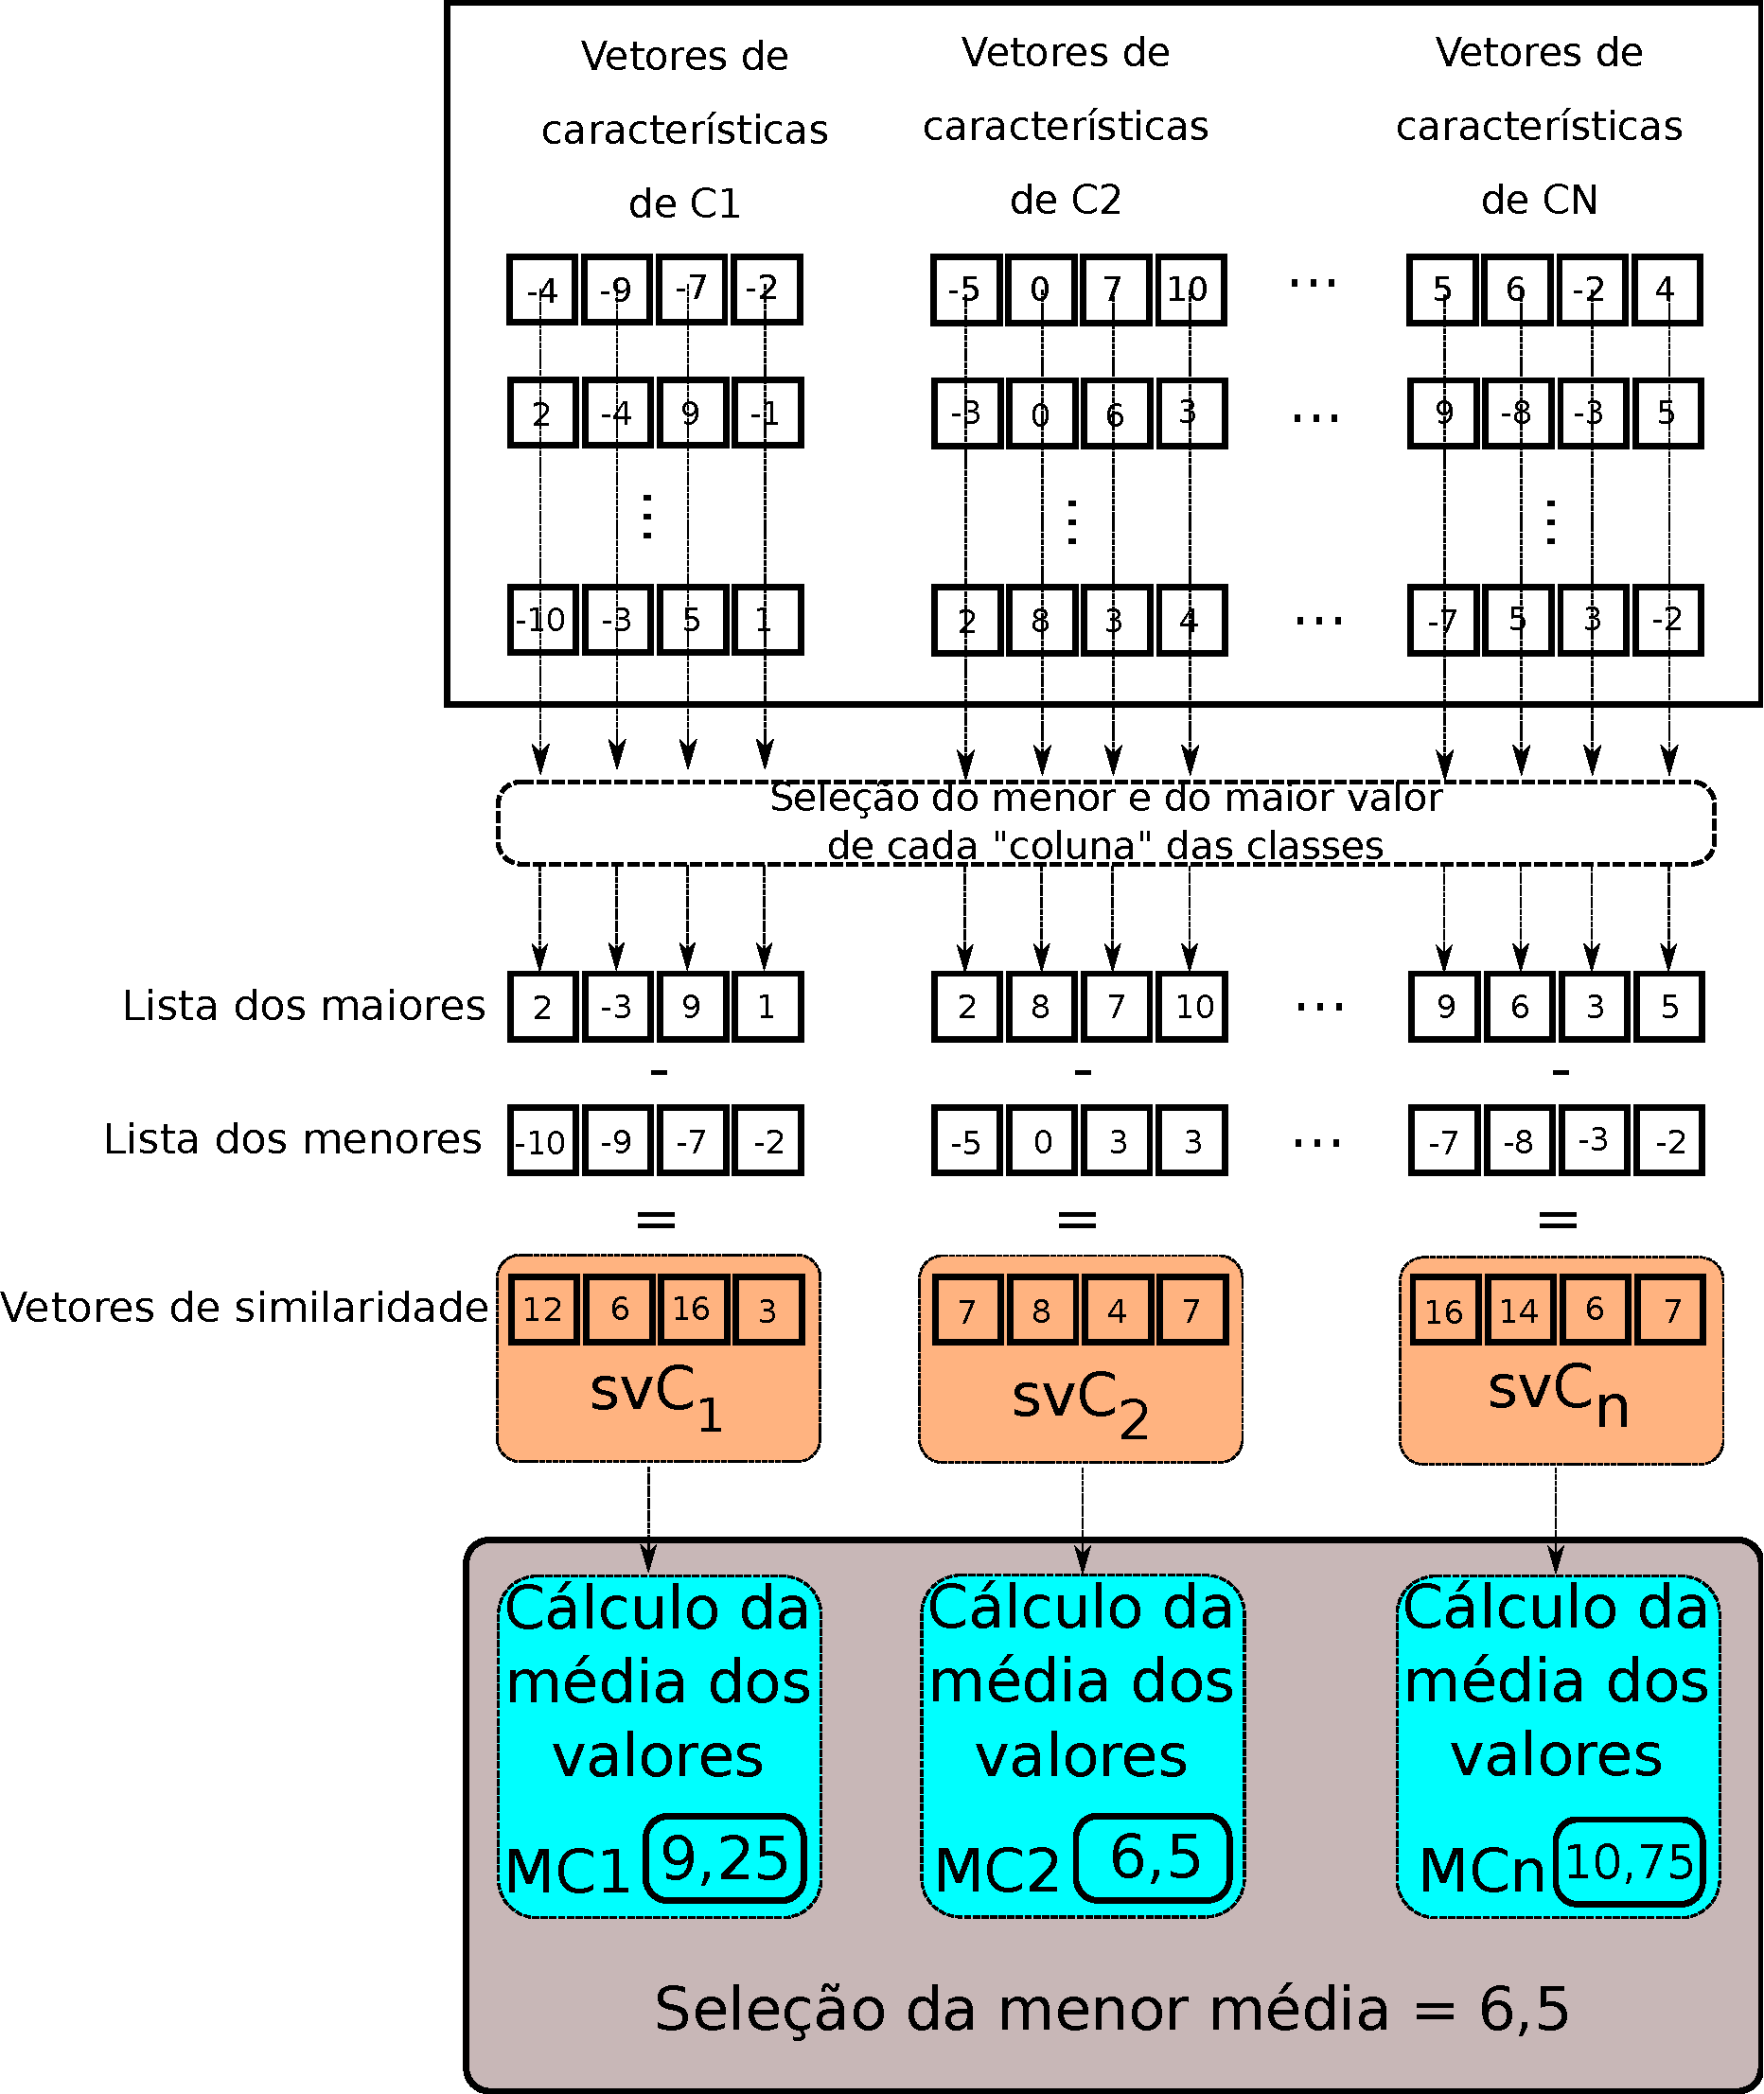
\includegraphics[width=0.5\linewidth]{images/calculoAlpha.pdf}
				\label{fig:calculoalpha}
				\legend{Adaptado de \cite{8588433}}
			\end{figure}
			
			\par A obtenção de $\beta$, assim como ilustrado na  \autoref{fig:betacalculation}, também se dá selecionando os maiores e os menores valores de cada uma das posições de todos os vetores de características de cada classe, gerando assim um vetor para os valores maiores e outro para os menores.
			
			\par Na sequência, realiza-se o cálculo de $R$ cujo valor é a quantidade de vezes que um valor do vetor de características de uma classe se encontra entre os valores maiores e menores de outra classe.
			
			\par Seja:
			\begin{itemize}
				\item N a quantidades de classes;
				\item X a quantidade de vetores de características por classe;
				\item T o tamanho do vetor de características.
			\end{itemize}
			
			\par Então, $F$, que é o número máximo de sobreposições possíveis entre classes, é dado por:
			\begin{equation}
				F=N.(N-1).X.T \qquad.
			\end{equation}
			\par Finalmente, $\beta$ é calculado da seguinte forma:
			\begin{equation}
				\beta=\dfrac{R}{F} \qquad.
			\end{equation}
	
			\par Neste ponto, é importante notar que $\alpha=1$ sugere fortemente que os vetores de características de cada classe são similares e representam suas respectivas classes precisamente. Complementarmente, $\beta=0$ sugere os vetores de características de classes diferentes não se sobrepõe \cite{8588433}.
			
			\begin{figure}[h]
				\centering
				\caption[Cálculo de $\beta$]{Cálculo de $\beta$: Os itens destacados em azul e rosa são aqueles pertencentes a classe C1 e CN que se sobrepõe, em verde, a sobreposição é entre C1 e C2. Para cada sobreposição verificada soma-se 1 ao valor $R$. Essa comparação é feita para todos os vetores de características de cada uma das classes.}
				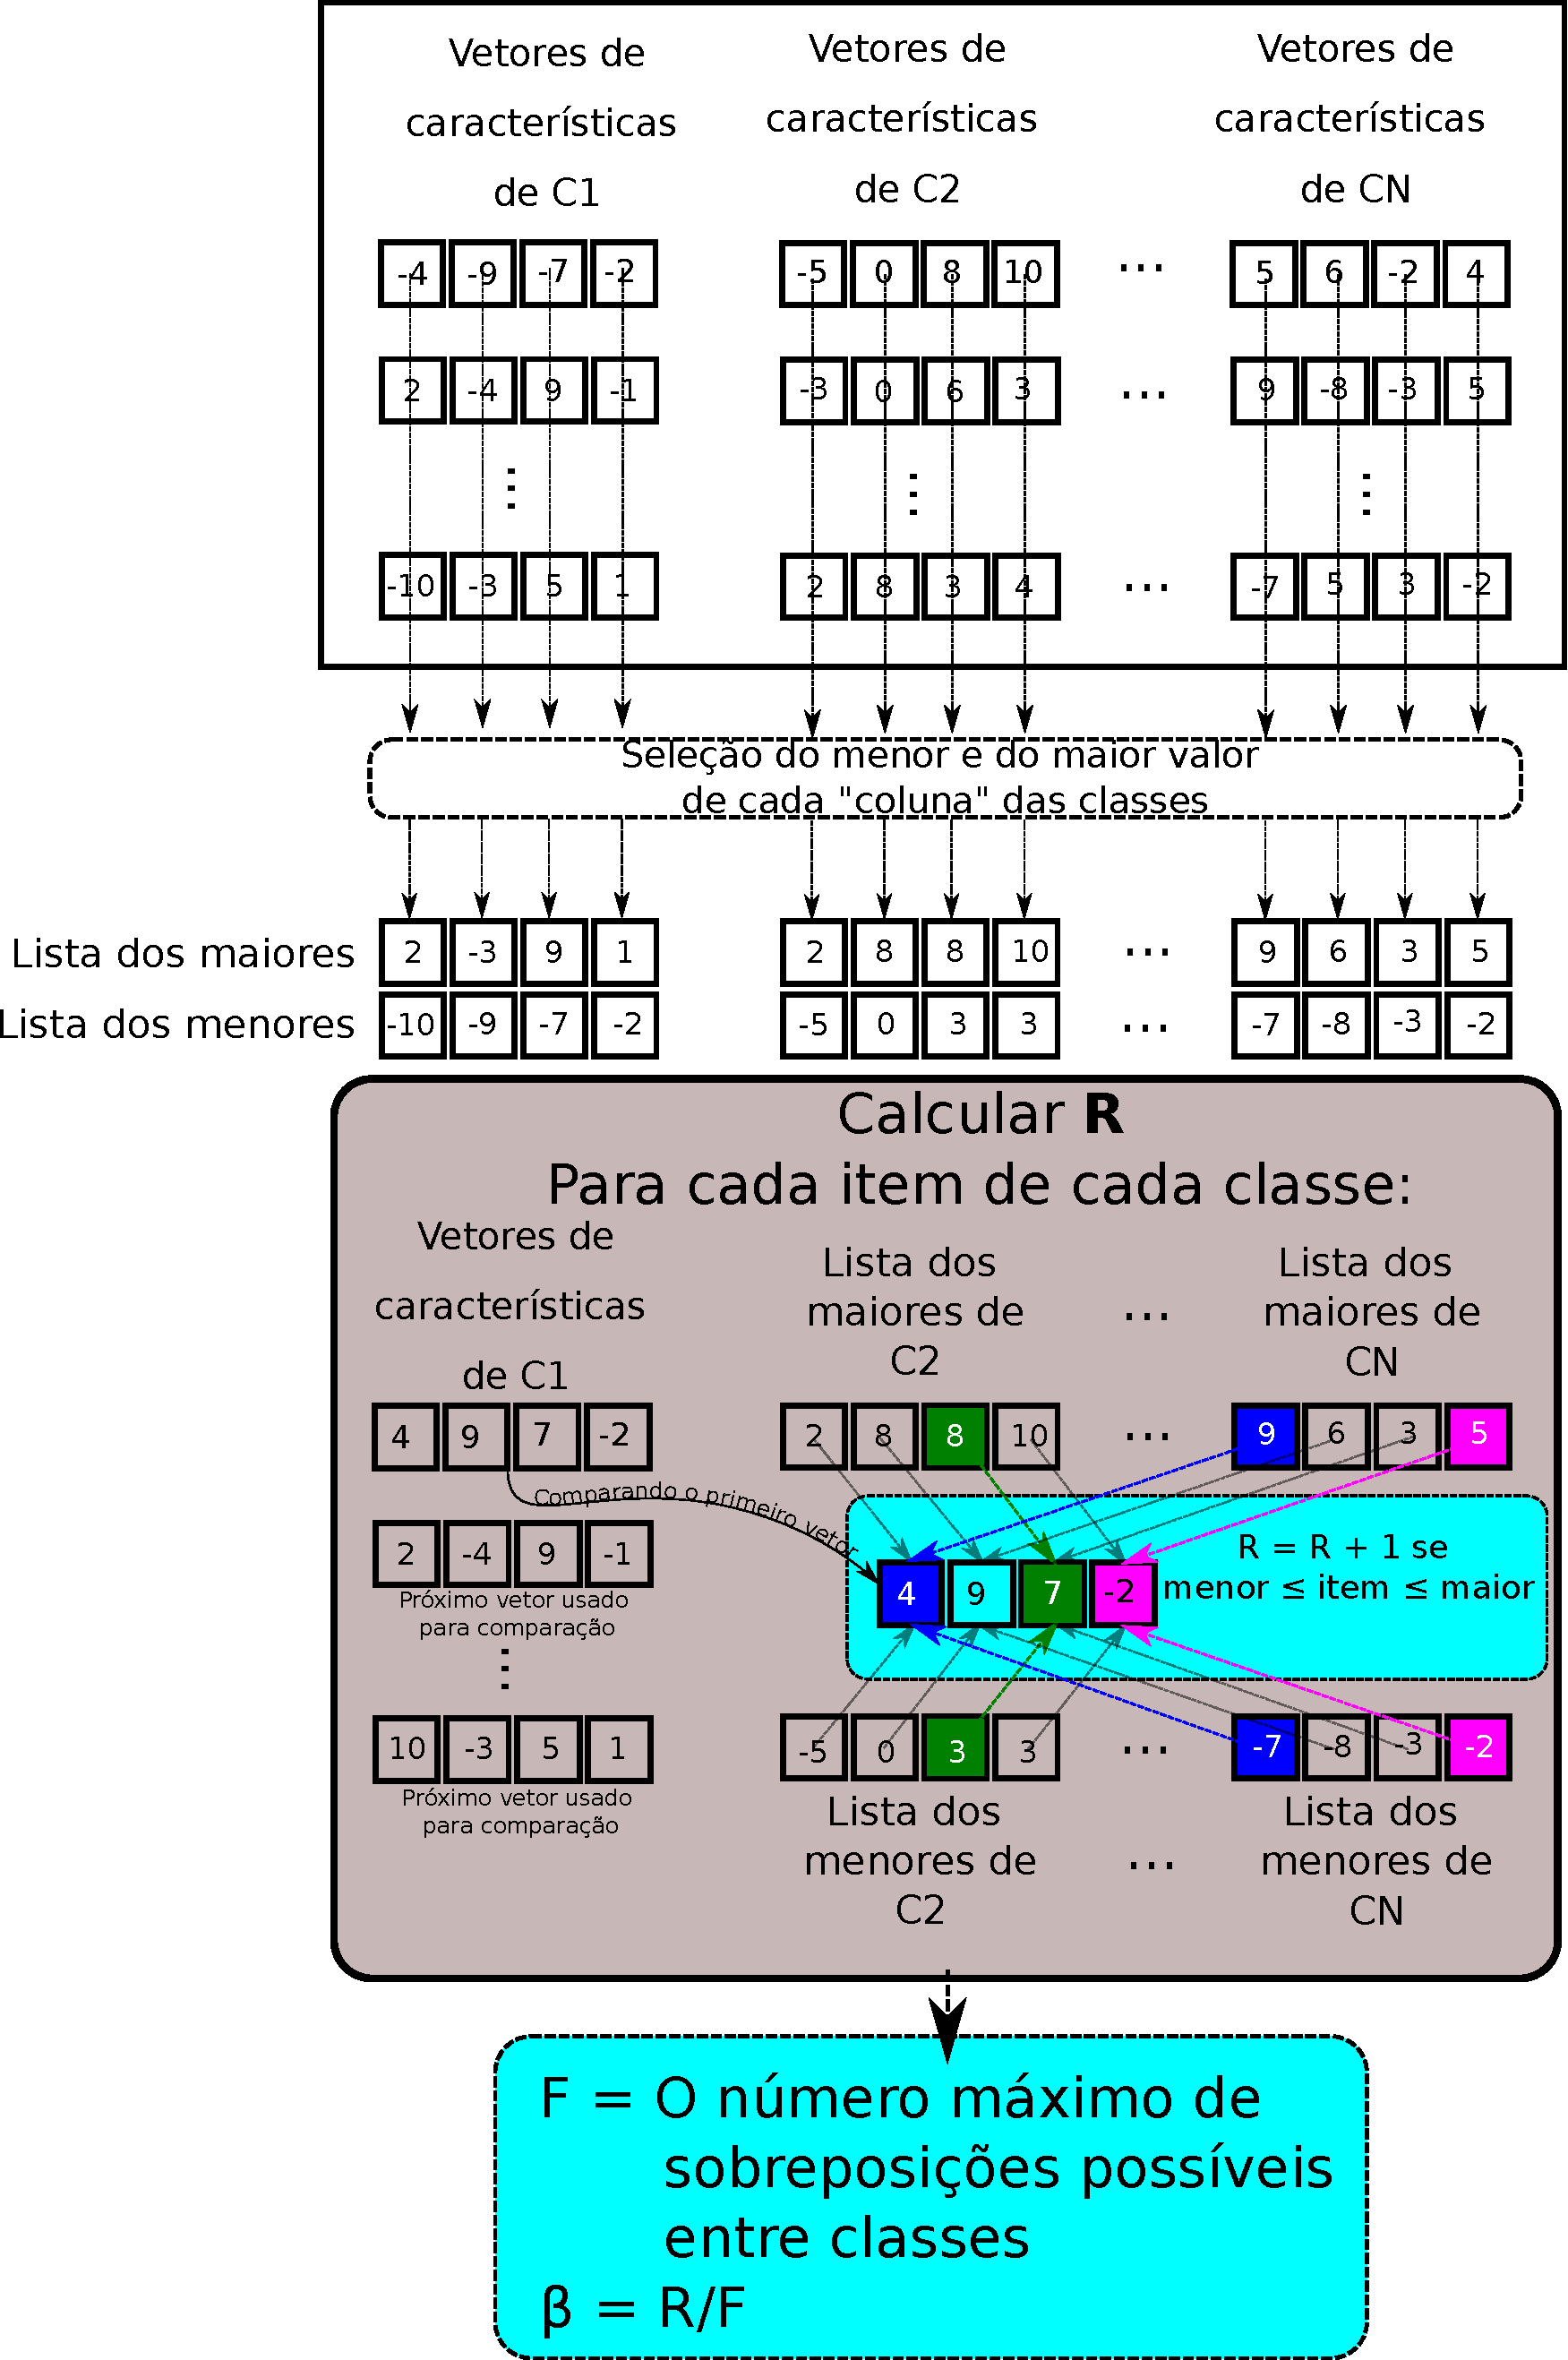
\includegraphics[width=0.5\linewidth]{images/betaCalculation.pdf}
				\label{fig:betacalculation}
				\legend{Adaptado de \cite{8588433}}
			\end{figure}
			
			\par Considerando-se o plano paraconsistente \cite{8588433}, temos: 
			
			\begin{itemize}
				\item Verdade $\rightarrow$ fé total ($\alpha = 1$) e nenhum descrédito ($\beta = 0$)
				\item Ambiguidade $\rightarrow$ fé total ($\alpha = 1$) e descrédito total ($\beta = 1$)
				\item Falsidade $\rightarrow$ fé nula ($\alpha = 0$) e descrédito total ($\beta = 1$)
				\item Indefinição $\rightarrow$ fé nula ($\alpha = 0$) e nenhum descrédito ($\beta = 0$) \qquad.
			\end{itemize}
	
			\par No entanto, raramente $\alpha$ e $\beta$ terão valores inteiros como os mostrados na listagem acima: Na maioria das ocasiões, $0 \leqslant \alpha \leqslant 1$ e $0 \leqslant \beta \leqslant 1$. Por isso, se torna necessário o cálculo do \textbf{grau de certeza}, isto é, $G_1$, e do \textbf{grau de contradição}, isto é, $G_2$, conforme segue:
			\begin{equation}
				G_1=\alpha-\beta  \qquad,
			\end{equation}
			\begin{equation}
				G_2=\alpha+\beta-1 \qquad,
			\end{equation}
			onde: $-1 \leqslant G_1$ e  $1 \geqslant G_2$.
			
			\par Os valores de $G_1$ e $G_2$, em conjunto, definem os graus entre verdade ($G_1=1$) e falsidade ($G_1=-1$) e também os graus entre indefinição ($G_2=-1$) e ambiguidade ($G_2=1$). Novamente, raramente tais valores inteiros serão alcançados já que $G_1$ e $G_2$ dependem de $\alpha$ e $\beta$.
	
			\par O Plano Paraconsistente, para fins de visualização e maior rapidez na avaliação dos resultados, encontra-se ilustrado na  \autoref{fig:paraconsistentplane} e tem quatro arestas precisamente definidas:
			\begin{itemize}
				\item (-1,0) $\rightarrow$ falsidade;
				\item (1,0) $\rightarrow$ verdade;
				\item (0,-1) $\rightarrow$ indefinição;
				\item (0,1) $\rightarrow$ ambiguidade.
			\end{itemize}
			\par A propósito de ilustração na  \autoref{fig:paraconsistentplane}, é possível ver um pequeno círculo indicando os graus dos quatro casos listados.
			
			\par Para se ter ideia em que área exatamente se encontram as classes avaliadas, as distâncias $(D)$ do ponto $P=(G_1,G_2)$ até o limites supracitados podem ser computadas. Tais cálculos podem ser feitos da seguinte forma:
	
			\begin{equation}
				D_{-1,0}=\sqrt{(G_1+1)^2+(G_2)^2}\qquad,
			\end{equation}
			\begin{equation}
				D_{1,0}=\sqrt{(G_1-1)^2+(G_2)^2}\qquad,
			\end{equation}
			\begin{equation}
				D_{0,-1}=\sqrt{(G_1)^2+(G_2+1)^2}\qquad,		
			\end{equation}
			\begin{equation}
				D_{0,1}=\sqrt{(G_1)^2+(G_2-1)^2}\qquad.
			\end{equation}		
			
			\begin{figure}[H]
				\centering
				\caption[O plano paraconsistente]{O plano paraconsistente: O pequeno círculo indica os graus de falsidade(-1,0), verdade(1,0), indefinição(0,-1) e ambiguidade(0,1)}
				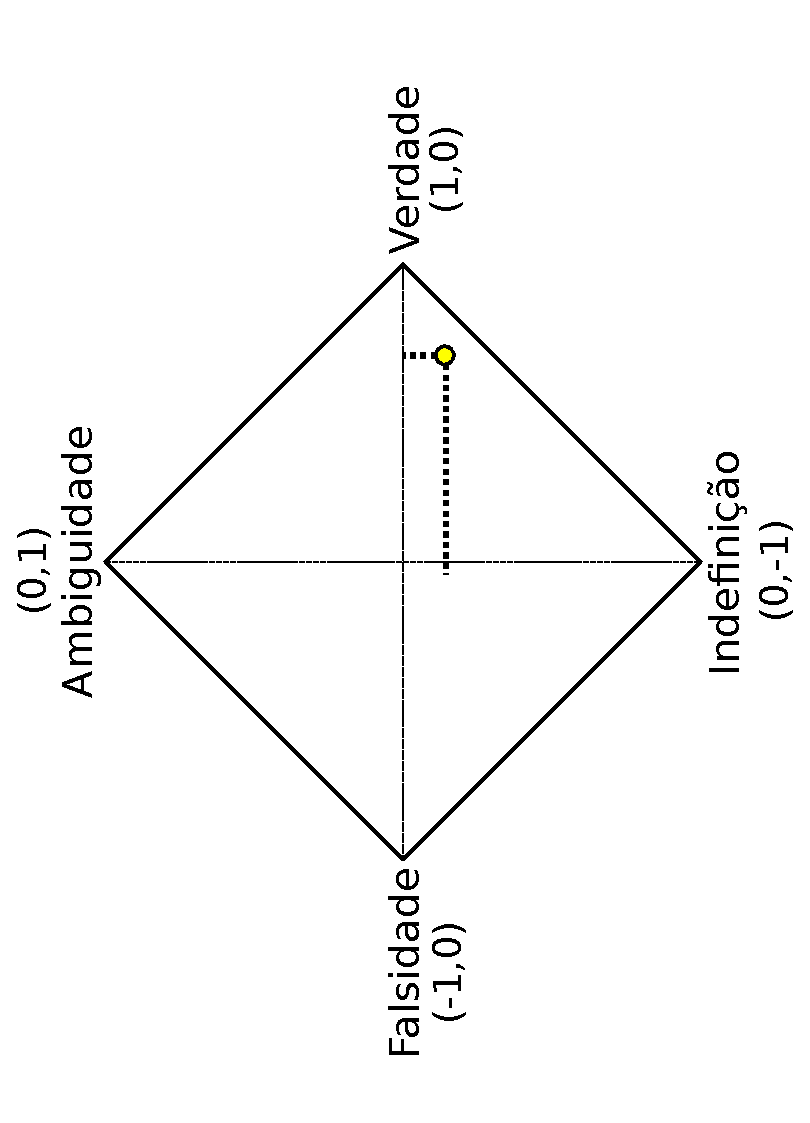
\includegraphics[angle=-90, width=0.69\linewidth]{images/paraconsistentPlane.pdf}
				\label{fig:paraconsistentplane}
				\legend{Adaptado de \cite{8588433}}
			\end{figure}
			\par Na prática, ou seja, para fins de classificação, geralmente considera-se a distância em relação ao ponto \textit{``(1,0) $\rightarrow$ Verdade''}, que é o ponto ótimo: quanto mais próximo o ponto $(G_1,G_2)$ estiver de $(1,0)$, mais as os vetores de características das diferentes classes estão naturalmente separados. Isso implica, dentro da limitação de cada algoritmo, em resultados melhores sejam quais forem os classificadores usados.
	
		\subsection{Interfaces Humano-Máquina e EEG}
			\label{subsec:BCIEEG}
			
			\par Entre os métodos de Interface Cérebro-Computador (BCI), o Eletroencefalograma (EEG) se destaca como o sistema mais econômico e simples de implementar. O EEG registra as atividades elétricas do cérebro captando-as através de eletrodos colocados ao longo do couro cabeludo. No entanto possui algumas peculiaridades como alta sensibilidade a interferência eletromagnética e dificuldade em capturar o sinal devido a posicionamentos subótimos dos eletrodos no couro cabeludo. Portanto, um dos aspectos fundamentais que qualquer sistema de processamento de EEG deve ter é a tolerância ao ruído \cite{JALALYBIDGOLY2020101788}.
			
			\par As atividades elétricas surgem dos fluxos de corrente iônica induzidos pela ativação sináptica sincronizada dos neurônios do cérebro. Elas se manifestam como flutuações de voltagem rítmicas com amplitude variando de 5 a 100$\mu V$ e frequência entre 0,5 e 40 Hz \cite{JALALYBIDGOLY2020101788}. Para cada tipo de ação realizada o cérebro trabalha segundo as bandas listadas em logo abaixo \cite{sanei2021eeg}.
			
			\par Para captação de sinais de EEG usam-se eletrodos que podem ser do tipo úmido ou seco. Os úmidos são colocados usando gel condutivo e são menos propensos a artefatos provocados por movimentos, que são interferências eletromagnéticas causadas, por exemplo, com o piscar dos olhos. Os eletrodos secos não precisam do gel, mas são mais sensíveis a tais artefatos.
			
			\begin{itemize}
				\item \textbf{Delta (1–4Hz)}: A onda mais lenta e geralmente a de maior amplitude. A banda Delta é observada em bebês e durante o sono profundo em adultos.
				
				\item \textbf{Theta (4–8Hz)}: Observada em crianças, adultos sonolentos e durante a recordação de memórias. A amplitude da onda Theta é tipicamente inferior a 100$\mu V$.
				
				\item \textbf{Alpha (8–12Hz)}: Geralmente a banda de frequência dominante, aparecendo durante a consciência relaxada ou quando os olhos estão fechados. A atenção focada ou a relaxamento com os olhos abertos reduzem a amplitude da banda Alpha. Essas ondas tem amplitudes normalmente inferiores a 50 $\mu V$.
				
				\item \textbf{Beta (12–25Hz)}: Associada ao pensamento, concentração ativa e atenção focada. A amplitude da onda Beta é normalmente inferior a 30 $\mu V$.
				
				\item \textbf{Gamma (acima de 25Hz)}: Observada durante o processamento sensorial múltiplo. Os padrões Gamma têm a menor amplitude.
				
			\end{itemize}
			
			\par As amplitudes das bandas Delta e Gamma não foram encontradas quando procuradas nas principais bases de dados.
			
			\par De acordo com \cite{JALALYBIDGOLY2020101788} e \cite{sistema10-20}, para a maioria das tarefas realizadas pelo cérebro, existem regiões associadas a elas, conforme visto na \autoref{tb:brainRegions}.
			
			\subsection{Sistema 10-20 e as áreas do cérebro}
			\begin{table}[H]
				\begin{center}
					\caption{Tarefas cerebrais e suas regiões correspondentes}
					\begin{tabular}{|c|c|p{0.4\textwidth}|}
						\hline
						Região & Canais & Tarefas\\
						\hline
						Lobo frontal & Fp1, Fp2, Fpz, Pz, F3, F7, F4, F8 & Memória, concentração, emoções.\\
						\hline
						Lobo parietal & P3, P4, Pz & Resolução de problemas, atenção, sentido do tato. \\
						\hline
						Lobo temporal & T3, T5, T4, T6 & Memória, reconhecimento de faces, audição, palavras e percepção social. \\
						\hline
						Lobo occipital & O1, O2, Oz & Leitura, visão.\\
						\hline
						Cerebelo && Controle motor, equilíbrio. \\
						\hline
						Córtex senso-motor & C3, C4, Cz& Atenção, processamento mental, controle motor fino, integração sensorial. \\
						\hline
					\end{tabular}
					\label{tb:brainRegions}
				\end{center}
			\end{table}
			
			\begin{figure}[H]
				\centering
				\caption[Sistema 10-20 e lobos cerebrais]{Posicionamento dos eletrodos de acordo com o padrão 10-20. Números ímpares são atribuídos aos eletrodos no hemisfério esquerdo, e números pares são atribuídos aos eletrodos no hemisfério direito.}
				\includegraphics[width=0.7\linewidth]{images/10–20StandardAndLobes}
				\legend{Fonte: \cite{JALALYBIDGOLY2020101788}}
				\label{fig:1020standardandlobes}
			\end{figure}
		
			\par Segundo \cite{bioengineering10060649} e \cite{pinto2012manual}, em se tratando da produção e articulação da fala, a área de Wernicke é responsável por garantir que a mesma faça sentido enquanto que a área de broca garante que seja produzida de forma fluente portanto, já que a investigação desse trabalho também envolve a fala fonada, uma atenção especial deve ser dada a essas regiões. De acordo com a \autoref{fig:loboparietal}, \autoref{fig:lobotemporal} e a \autoref{fig:1020standardandlobes} os eletrodos frontais e temporais esquerdos F7 e T5 podem estar mais próximos da área de Wernicke e os eletrodos Fp1, F3 e F7 da área de Broca.
			%TODO Noo entanto a fala imaginada ocorre em todo o cérebro, citar fontes.
			%TODO citar \cite{doi:10.1073/pnas.1414491112} e \cite{DeWitt_Rauschecker_2013} ?
			
			\begin{figure}[H]
				\centering
				\caption[Lobos Frontal, Parietal, Occipital e Temporal]{Principais regiões do cérebro: Lobos Frontal, Parietal, Occipital e Temporal}
				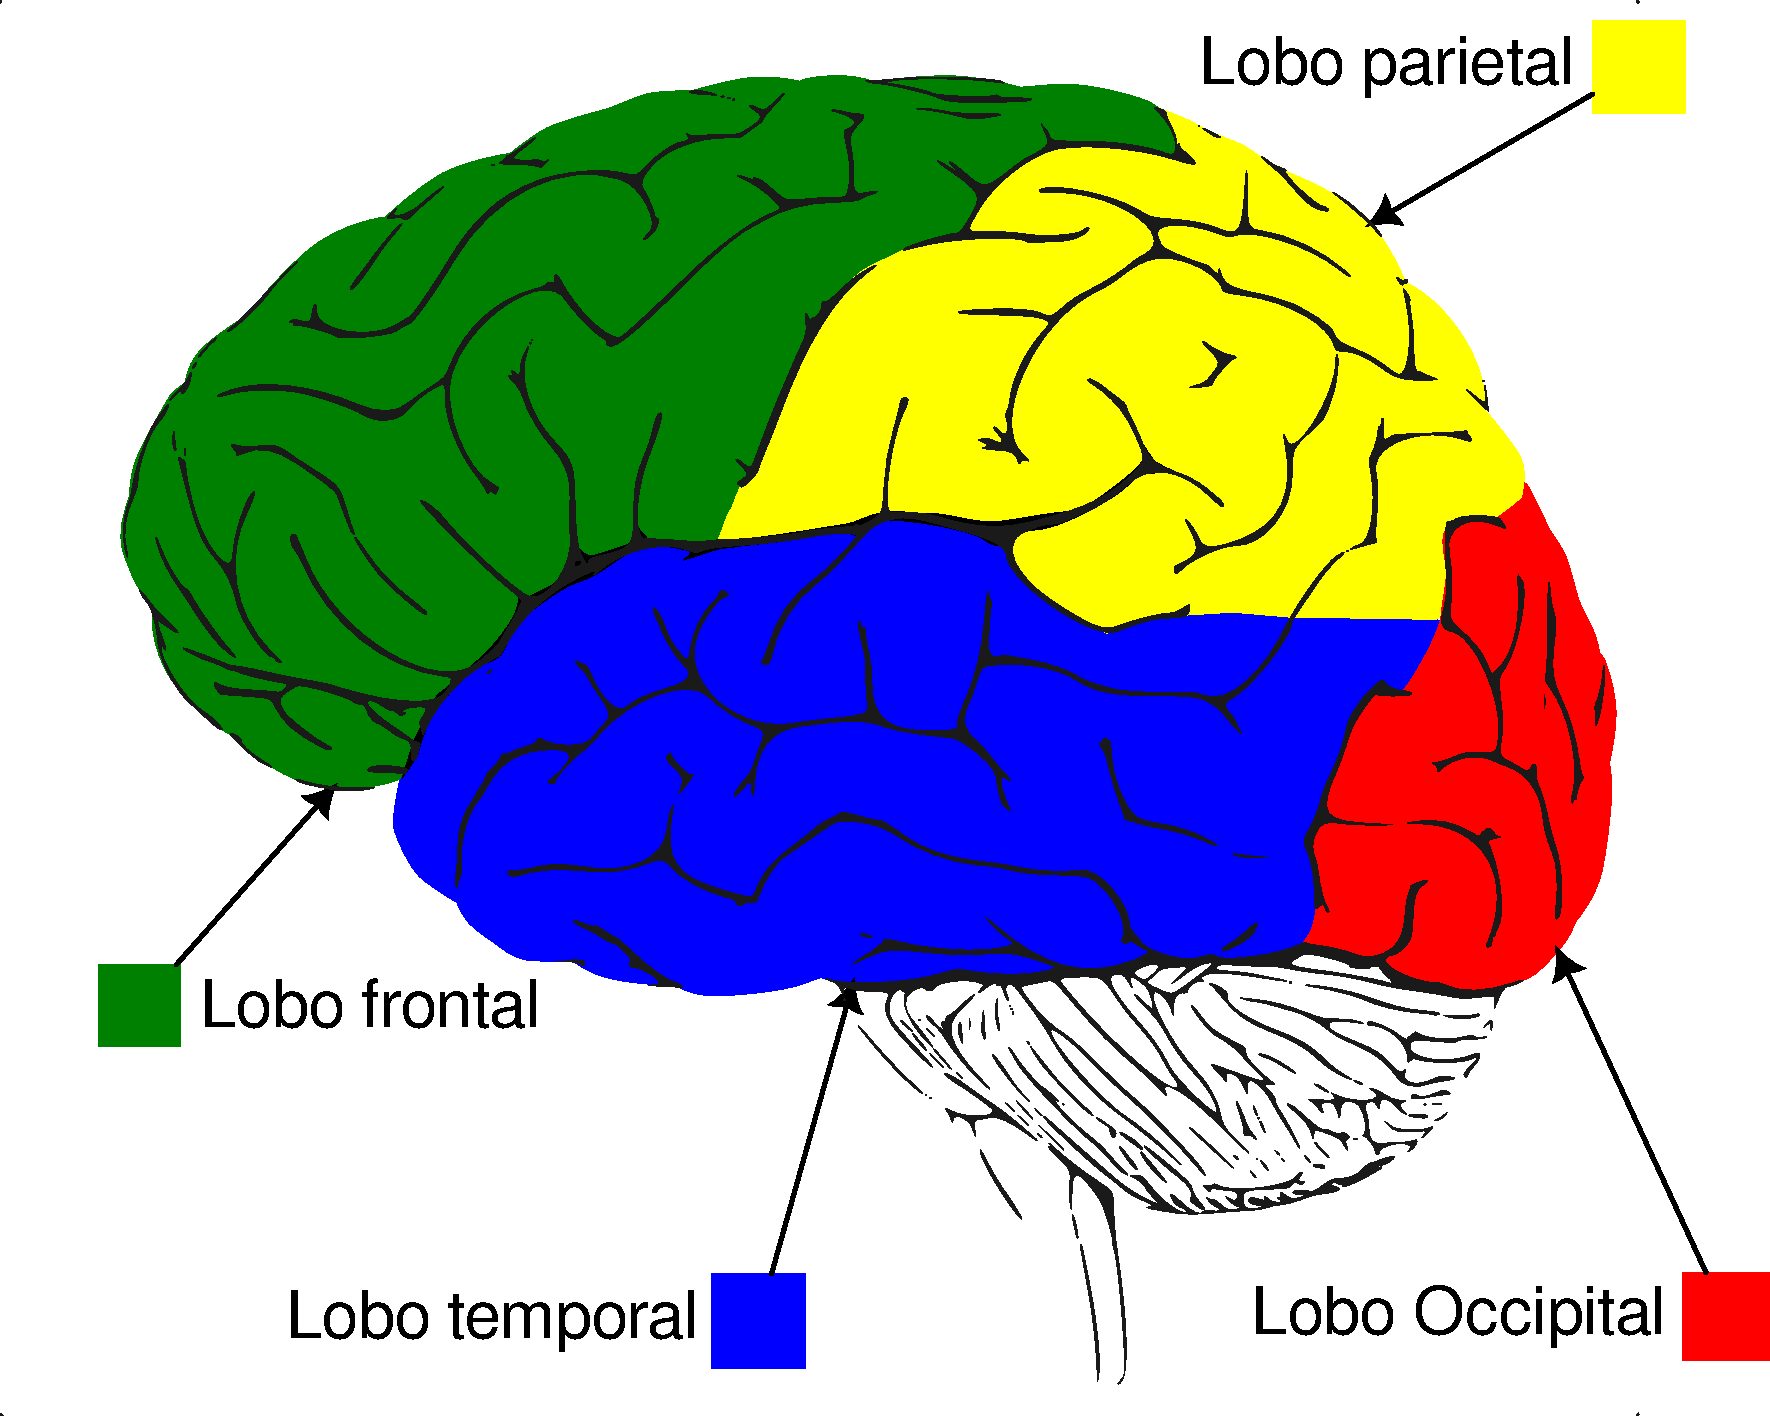
\includegraphics[width=0.65\linewidth]{images/lobosTelencefalo}
				\legend{Fonte: Elaborado pelo autor}
				\label{fig:lobostelencefalo}
			\end{figure}
			
			\begin{figure}[H]
				\centering
				\caption[Lobo frontal]{Áreas relacionadas a fala no lobo frontal: A área de Broca geralmente se encontra no hemisfério esquerdo.}
				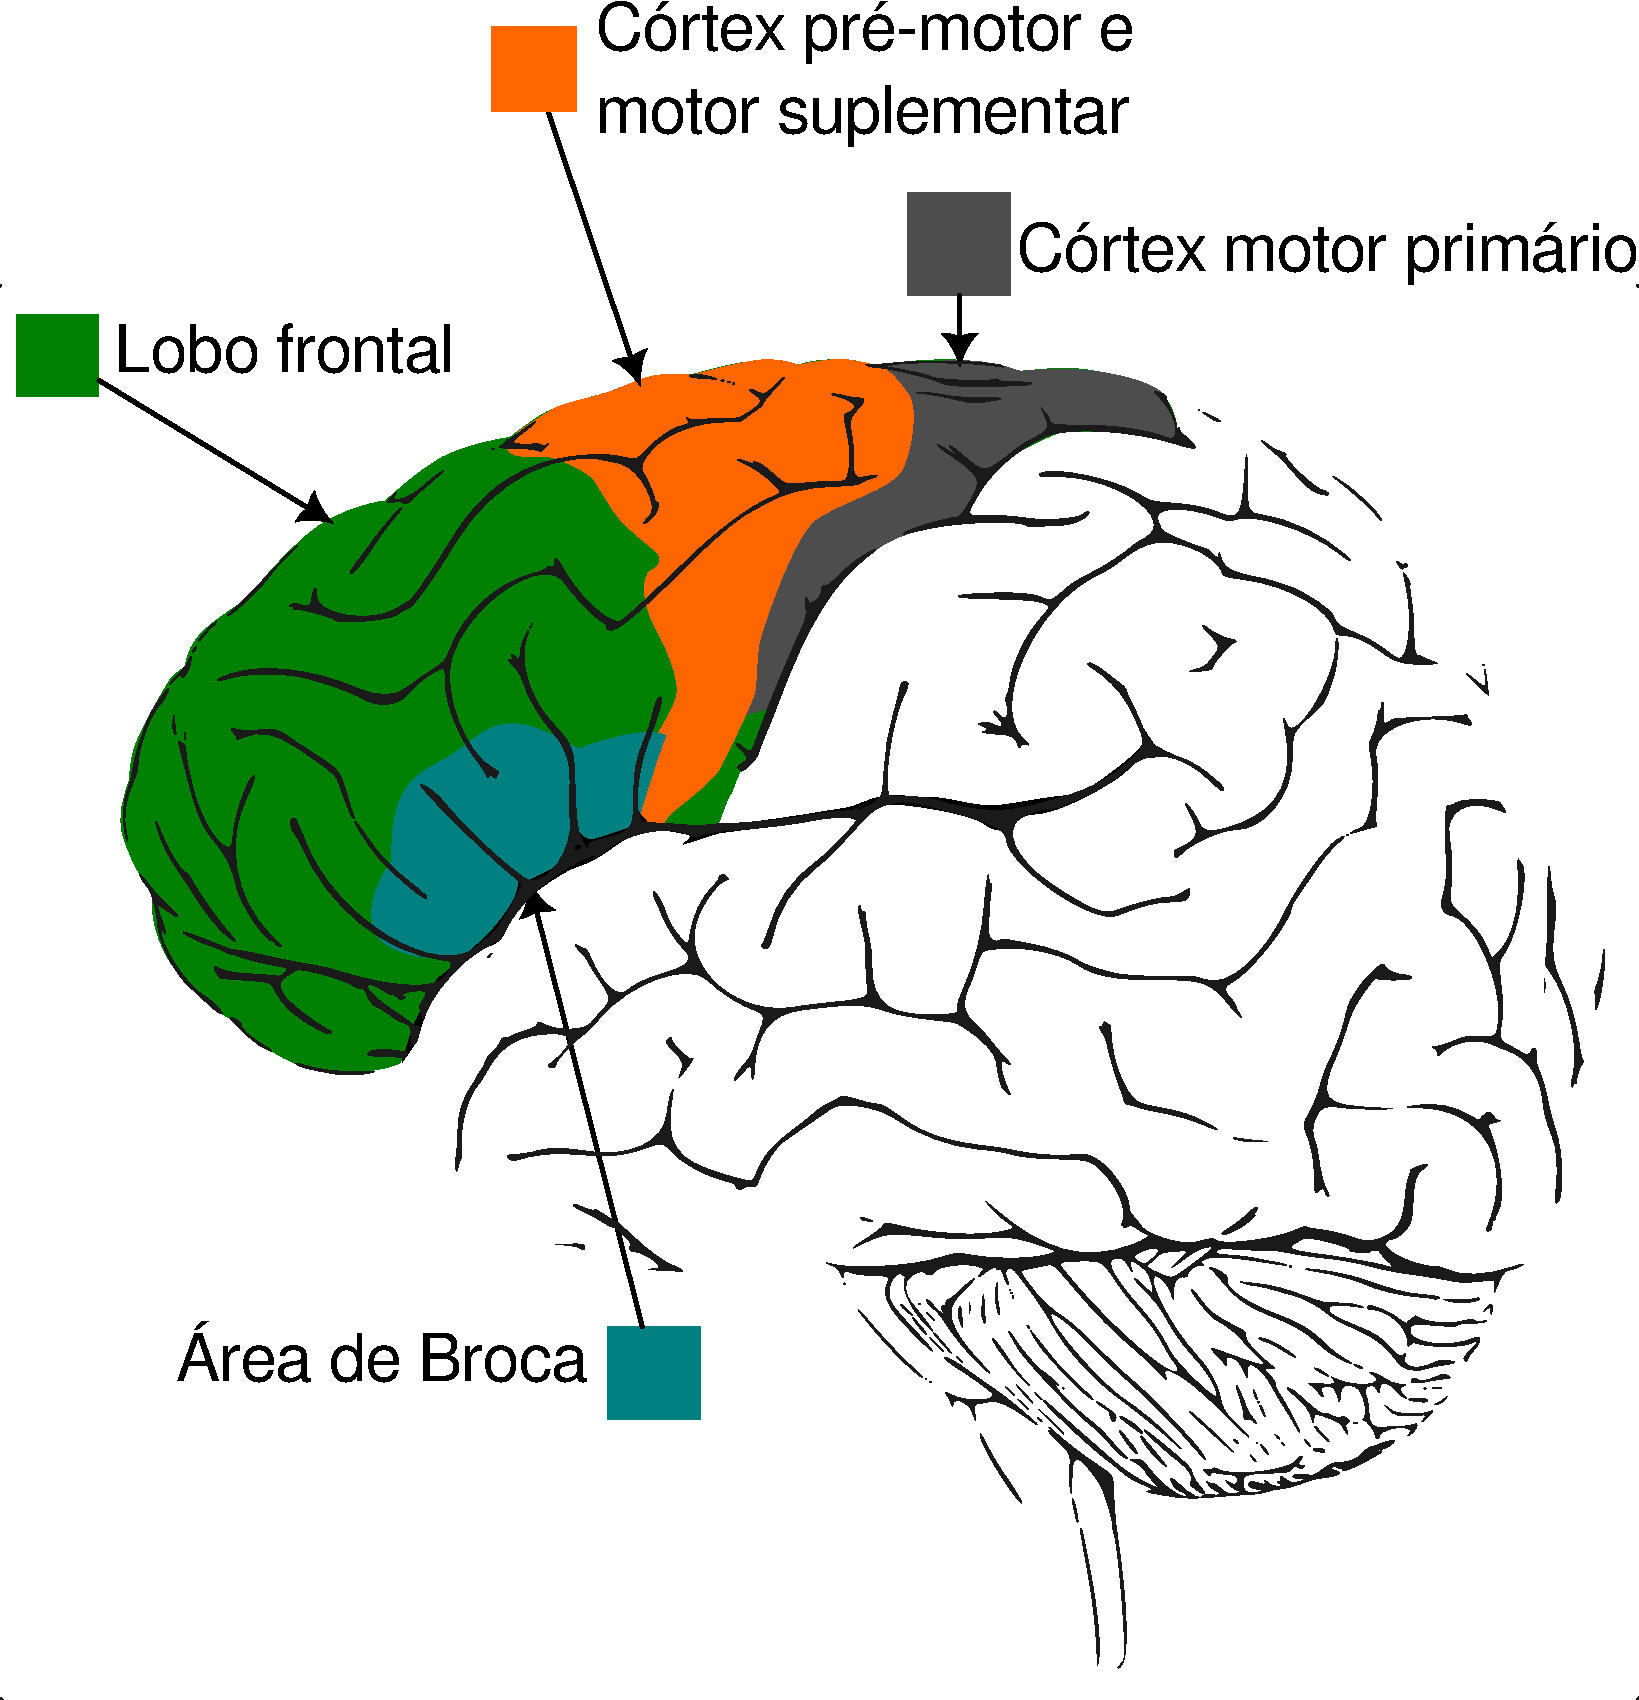
\includegraphics[width=0.65\linewidth]{images/loboFrontal}
				\legend{Fonte: Elaborado pelo autor}
				\label{fig:lobofrontal}
			\end{figure}
			\newpage
			
			\begin{figure}[H]
				\centering
				\caption[Lobo parietal]{Áreas relacionadas a fala no lobo parietal: A área de Wernicke também ocupa parte do lobo temporal e geralmente se encontra no hemisfério esquerdo.}
				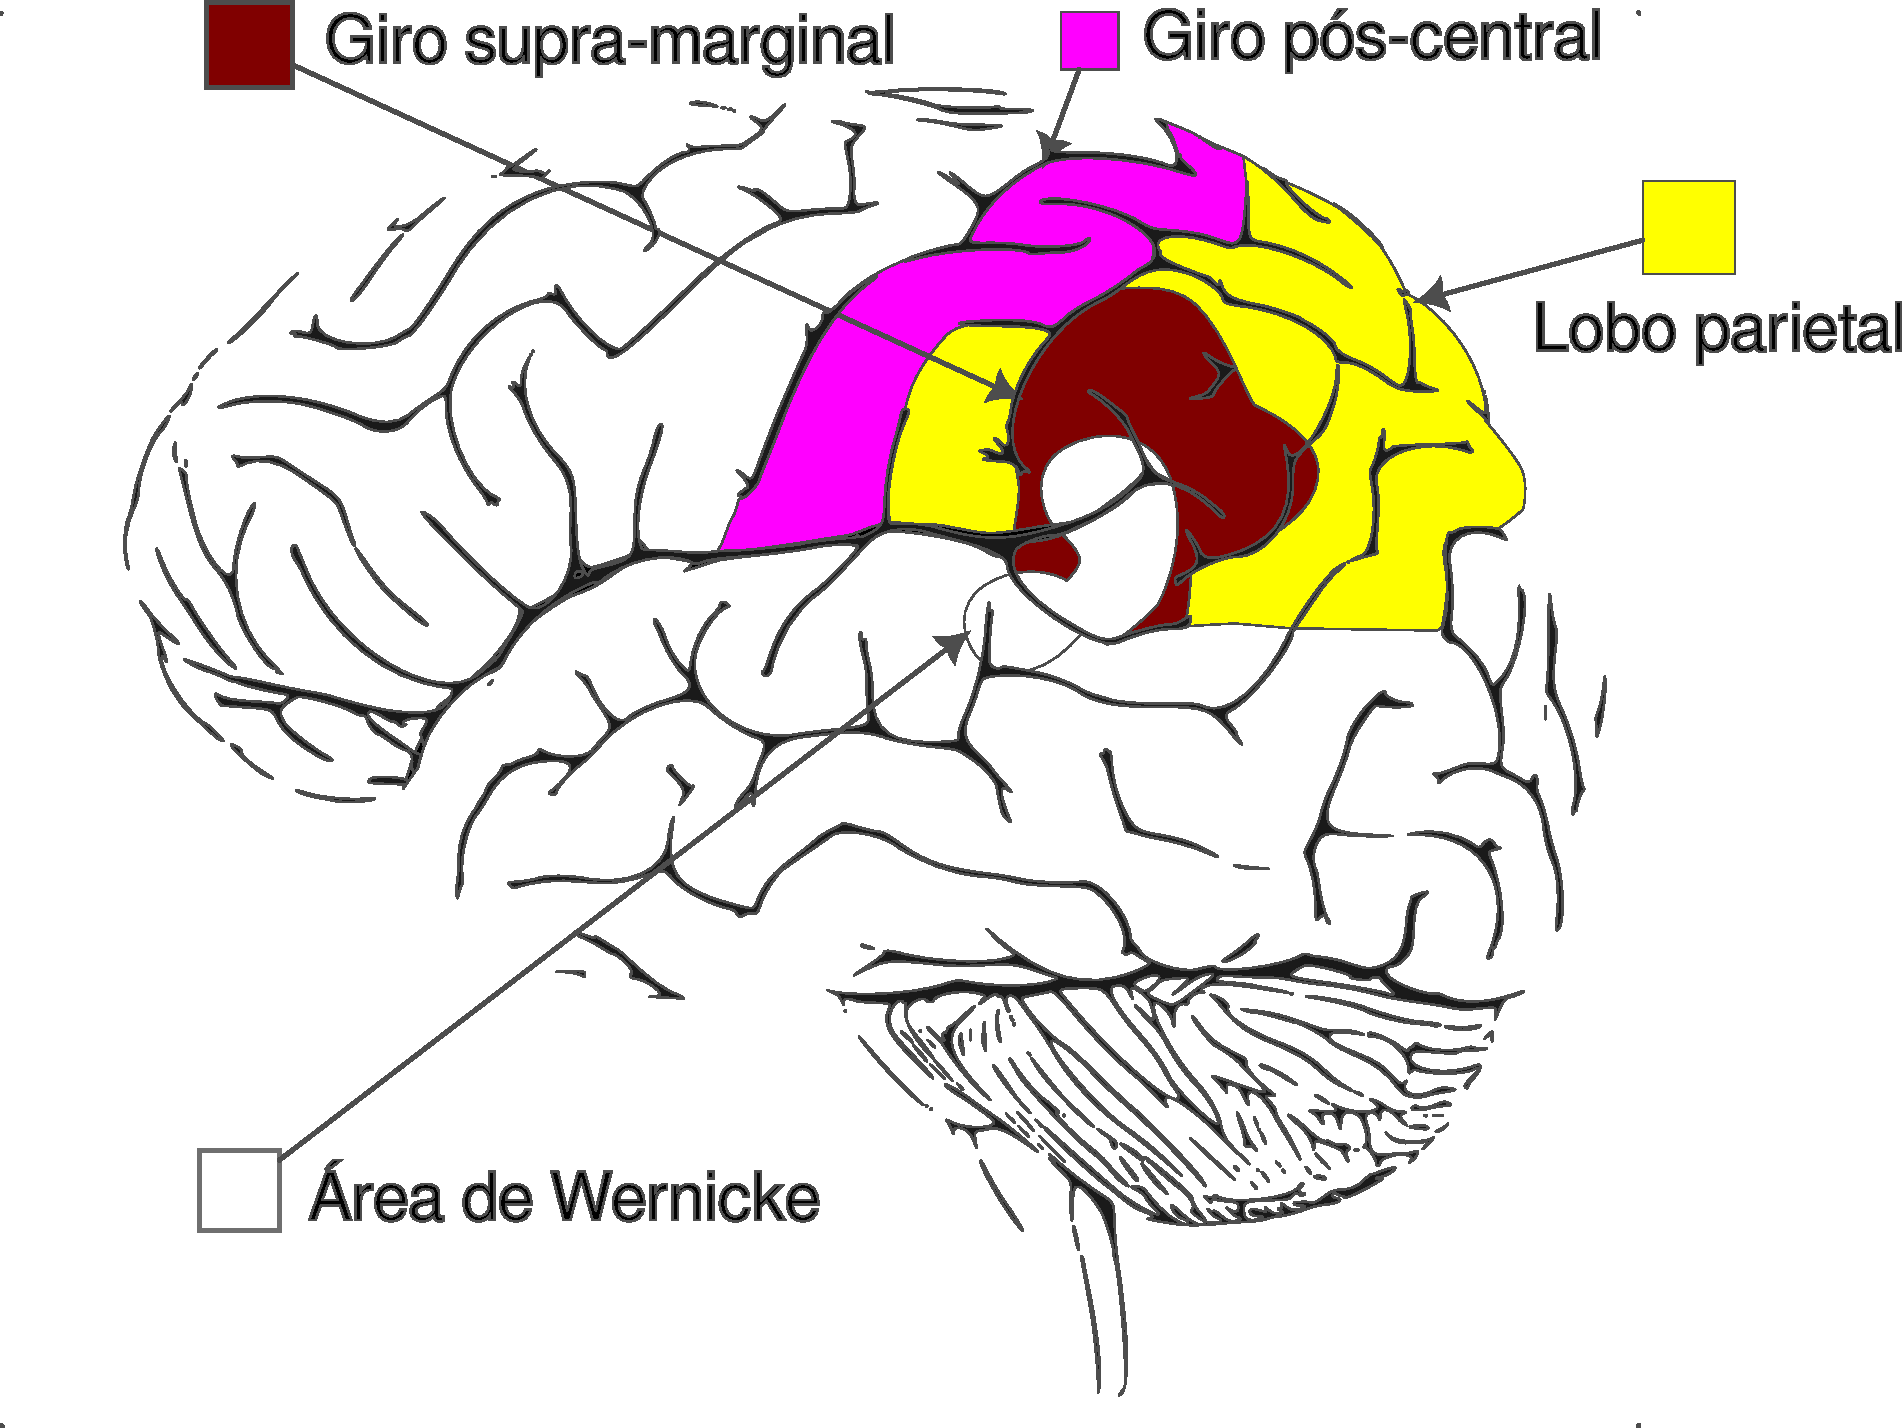
\includegraphics[width=0.72\linewidth]{images/loboparietal}
				\legend{Fonte: Elaborado pelo autor}
				\label{fig:loboparietal}
			\end{figure}
			
			\begin{figure}[H]
				\centering
				\caption[Lobo temporal]{Áreas relacionadas a fala no lobo temporal: A área de Wernicke também ocupa parte do lobo parietal e geralmente se encontra no hemisfério esquerdo.}
				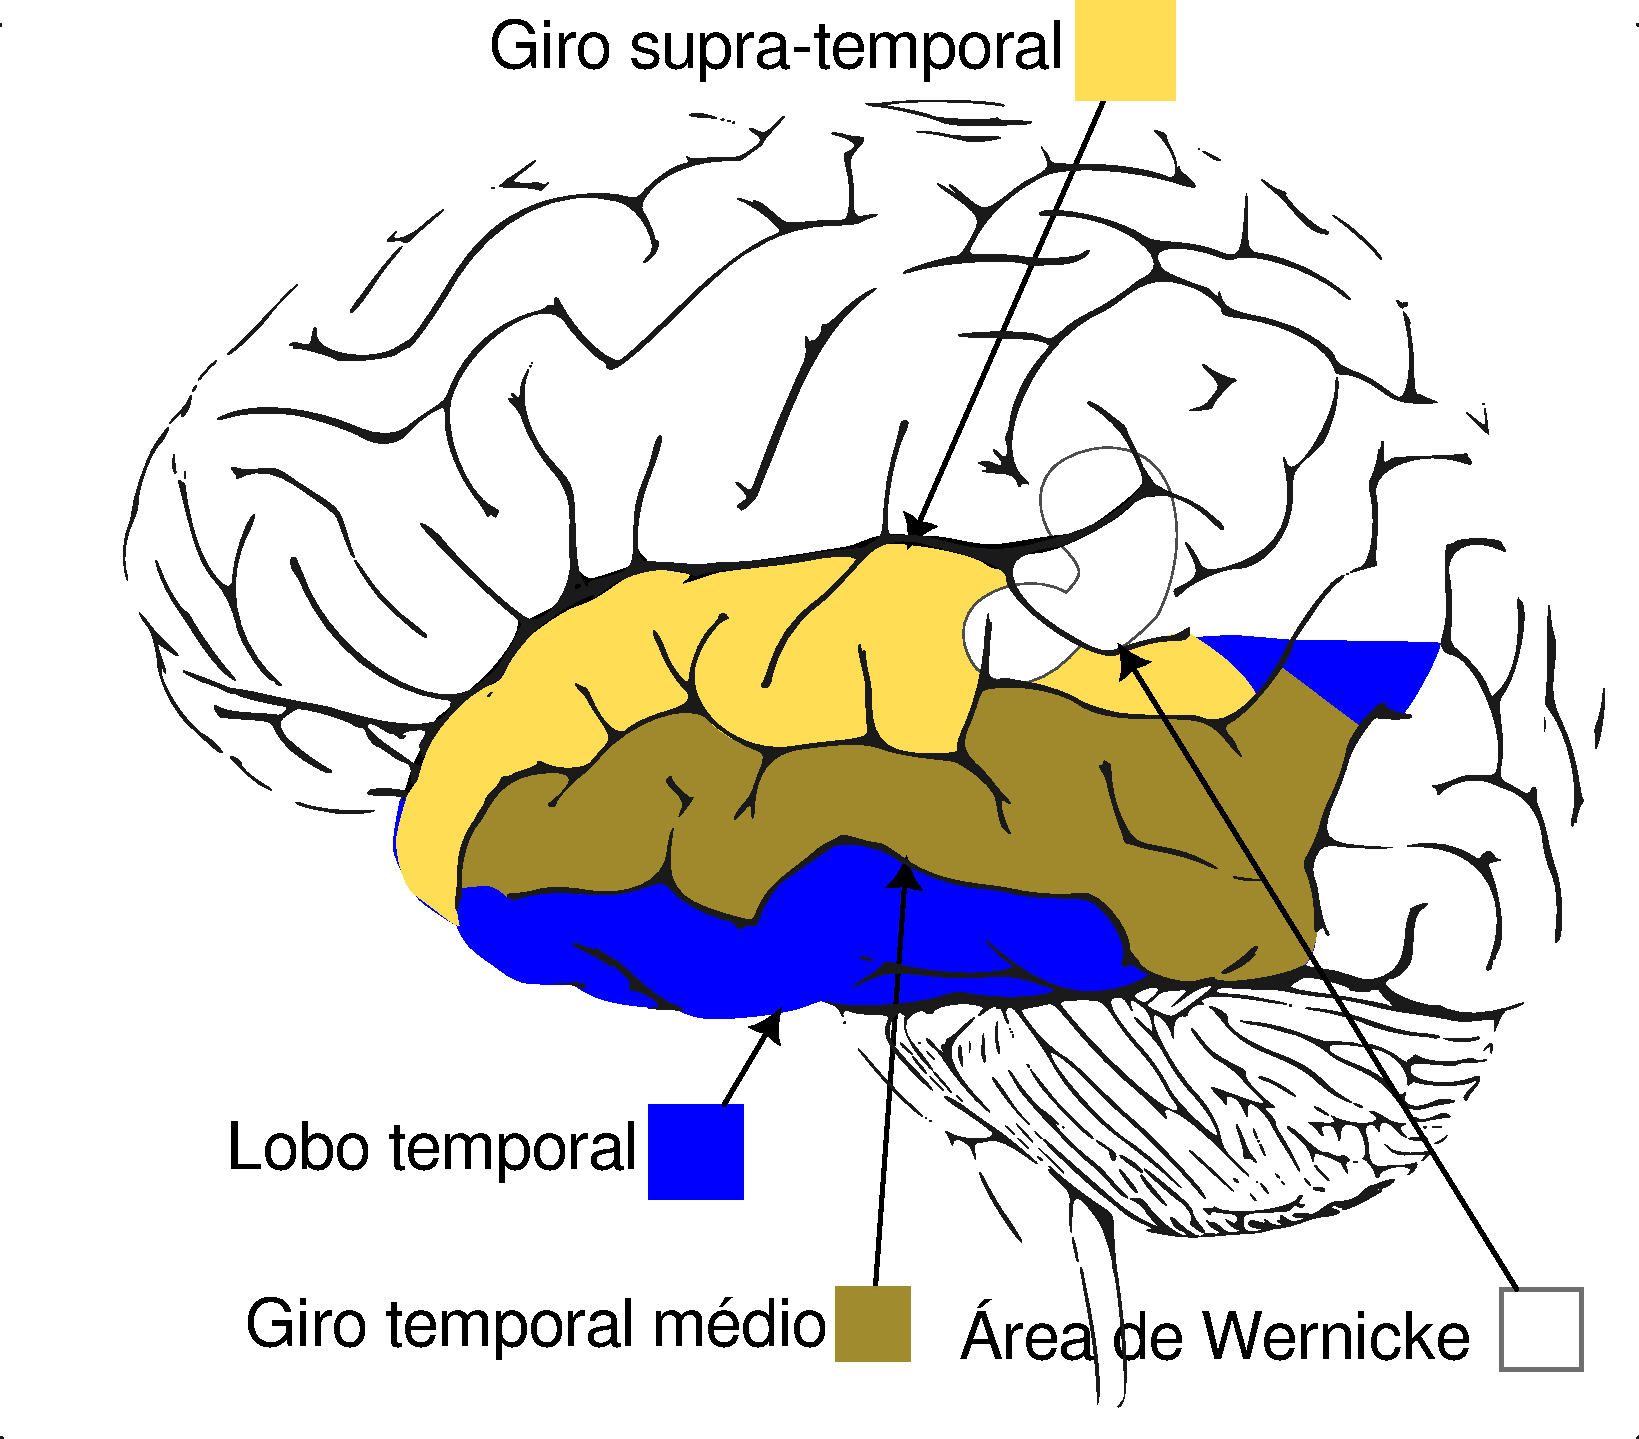
\includegraphics[width=0.72\linewidth]{images/loboTemporal}
				\legend{Fonte: Elaborado pelo autor}
				\label{fig:lobotemporal}
			\end{figure}
			
			\begin{figure}[p]
				\centering
				\caption[Visão geral do telencéfalo]{Visão geral do telencéfalo e as áreas relacionadas à fala, é interessante notar que tais regiões avizinham-se da fissura de Sylvius, sendo então chamadas de perissilvianas \cite{pinto2012manual}}
				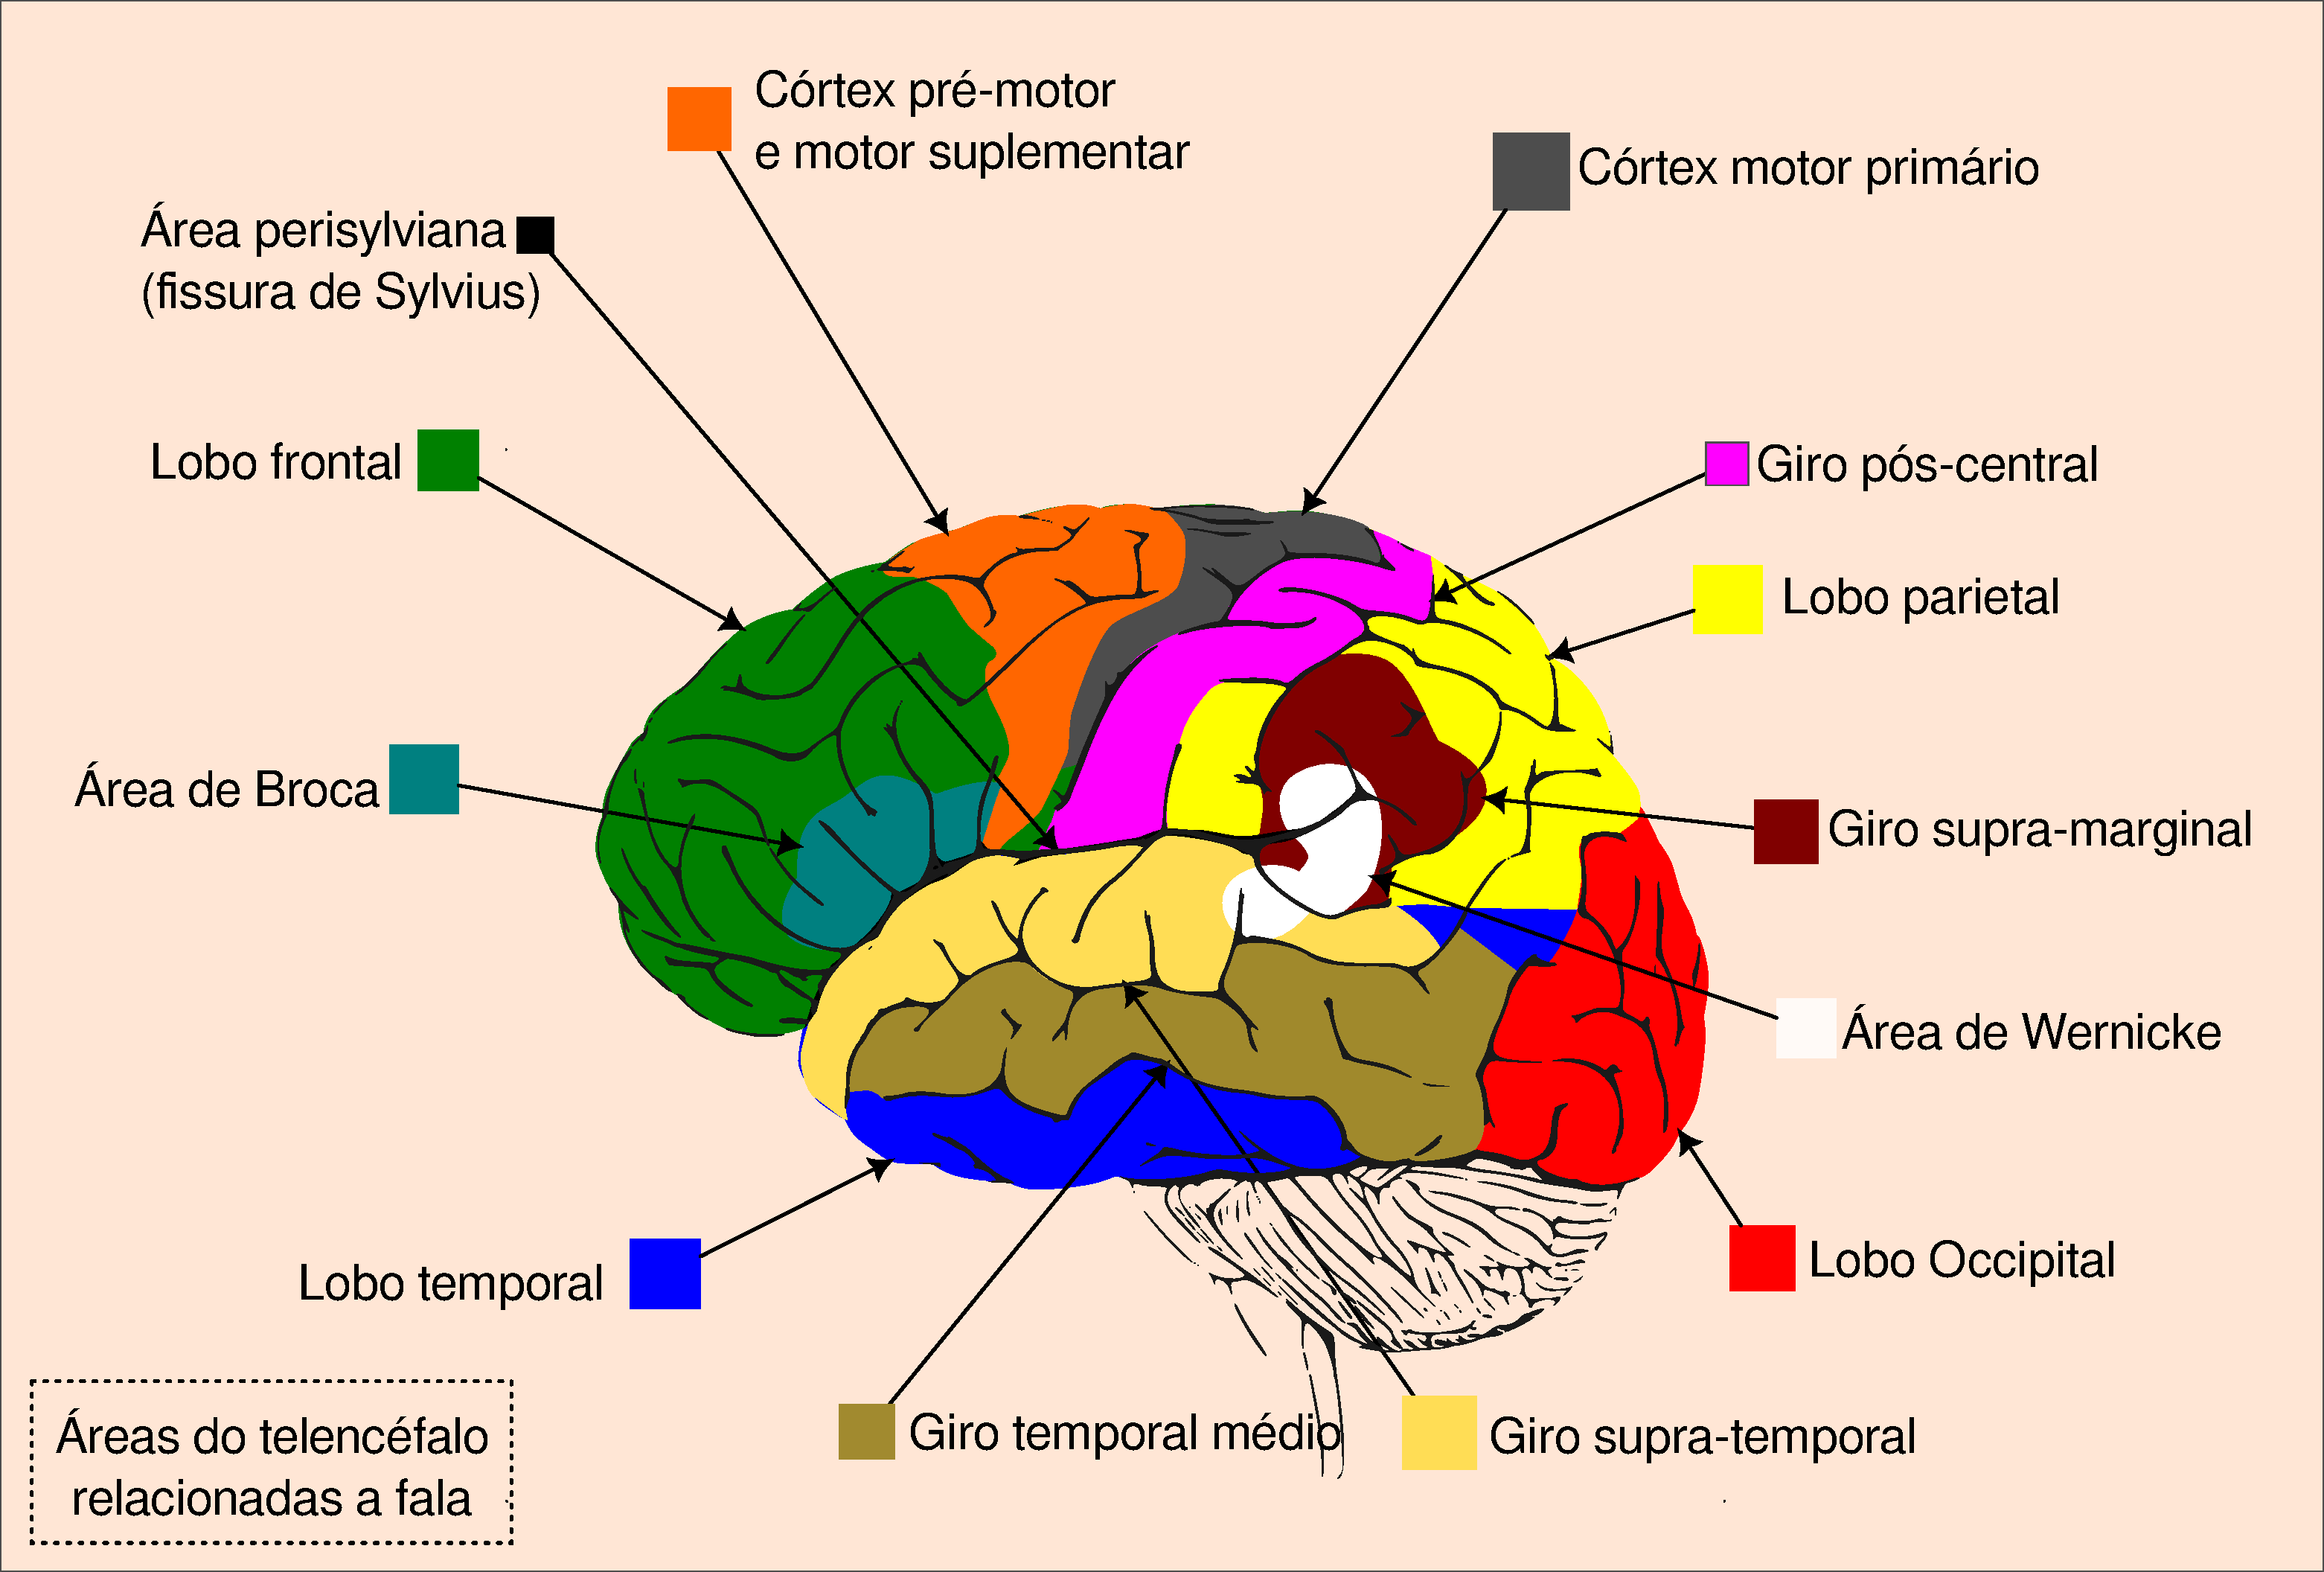
\includegraphics[angle=-90,width=.76\paperwidth,keepaspectratio]{images/teleencefaloTudo}
				\legend{Fonte: Elaborado pelo autor}
				\label{fig:teleencefalotudo}
			\end{figure}
			
			\par O processamento fonológico se dá na região perissilviana do hemisfério dominante, já o semântico inclui áreas corticais de ambos os hemisférios para dar significado as palavras, nas áreas frontais, temporais e parietais a articulação das palavra acontece. Quando se dá uma lesão em áreas como a de Wernicke, Broca ou em suas vizinhanças à condição resultante se dá o nome de \textbf{afasia} \cite{pinto2012manual}. Portanto  a fala tanto fonada quanto imaginada se realiza em quase todo o telencéfalo tendo como diferença a mobilização dos córtex motores quando o locutor ou locutora emite algum som.
			
			\begin{figure}[h]
				\centering
				\caption[Afasias e seus sintomas]{Afasias e seus sintomas: Sendo C.O. a compreensão oral. As afasias são resultado de lesões: Na área de Broca (Afasia de Broca), nas regiões superiores ou anteriores a área de Broca (Afasia transcortical motora), na área de Wernicke (Afasia de Wernicke) e finalmente ao redor da área de Wernicke (Afasia transcortical sensorial).}
							\begin{tikzpicture}[
	level 1/.style={level distance=20mm, sibling distance=80mm},
	level 2/.style={level distance=20mm, sibling distance=50mm},
	level 3/.style={level distance=20mm, sibling distance=25mm},
	edge from parent/.style={
		->,
		draw,
		line width=1.5pt % Adjust the line width here
	},
	>=latex,
	every node/.style={
		rectangle, 
		draw=none, 
		align=center, 
		rounded corners,
		inner sep=5pt,
		fill=green!70!black, text=black
	},
	% Style for the last level
	last_level_style/.style={
		fill=blue!70!black, % Change color here
		text=white
	}
	]
	\node {Afasias}
	child {
		node {Não fluentes}
		child {
			node {\shortstack{C.O\\preservada}}
			child {
				node {\shortstack{Repetição\\prejudicada}}
				child {
					node[last_level_style] {\shortstack{Afasia de\\Broca}}
				}
			}
			child {
				node {\shortstack{Repetição\\preservada}}
				child {
					node[last_level_style] {\shortstack{Afasia \\transcortical \\motora}}
				}
			}
		}
	}
	child {
		node {Fluentes}
		child {
			node {\shortstack{C.O\\prejudicada}}
			child {
				node {\shortstack{Repetição\\prejudicada}}
				child {
					node[last_level_style] {\shortstack{Afasia de \\Wernicke}}
				}
			}
			child {
				node {\shortstack{Repetição\\preservada}}
				child {
					node[last_level_style] {\shortstack{Afasia \\transcortical \\sensorial}}
				}
			}
		}
		child {
			node {\shortstack{C.O\\preservada}}
			child {
				node {\shortstack{Repetição\\prejudicada}}
				child {
					node[last_level_style] {\shortstack{Afasia de \\condução}}
				}
			}
			child {
				node {\shortstack{Repetição\\preservada}}
				child {
					node[last_level_style] {\shortstack{Afasia \\anômica}}
				}
			}
		}
	};
\end{tikzpicture}
				\legend{Fonte: Adaptado de \cite{pinto2012manual}.}
			\end{figure}


		\subsection{Redes Neurais de Pulso (Spiking Neural Networks)}
			
			\par Redes Neurais (RNs), conforme definido aqui como \textit{uma rede multicamadas, totalmente conectada, com ou sem camadas recorrentes ou convolucionais}, exigem que todos os neurônios sejam ativados tanto na fase de \textit{feed-forward} quanto na de \textit{backpropagation}. Isso implica que cada unidade na rede deve processar alguns dados, resultando em consumo de energia \cite{10242251}.
			
			\par Em contrapartida o neurônio biológico dispara apenas quando um certo nível de sinais excitatórios (voltagem) se acumula acima de um limiar em seu citoplasma, permanecendo inativo quando não há sinal, portanto, esse tipo de processamento é muito eficiente em termos de consumo de energia.

			\par O sistema sensorial dos sistemas neurológicos biológicos converte dados externos, como luz, odores, toque, sabores e outros, em pulsos. Um pulso é uma alteração na voltagem que é propagada transmitindo informações \cite{kasabov2019time}. Esses pulsos são então transmitidos ao longo da cadeia neuronal sendo processados, gerando uma resposta ao ambiente.
			
			\par Sendo assim, para obter as vantagens mencionadas, as Redes Neurais de Pulso (RNP) assim como seus referenciais biológicos, em vez de empregar valores de ativação contínuos, como as RNs, utilizam \textbf{pulsos} nas camadas de entrada, ocultas e de saída. As RNPs também podem ter entradas contínuas e manter suas propriedades.
			
			\par Uma RNP \textbf{não é} uma simulação um-para-um de neurônios. Em vez disso, ela aproxima certas capacidades computacionais de propriedades biológicas específicas. Caso haja interesse em algo do tipo existem modelos mais biologicamente precisos como o \textbf{neurônio Hodgkin-Huxley} \cite{gerstner2014neuronal} ou ainda outros que exploram a não linearidade dos dendritos e outras características neurais \cite{jones2020single} criando modelos muito mais próximos aos neurônios naturais, obtendo resultados bastante interessantes.
			
			\par Como pode ser visto na \autoref{fig:neuronspike}, os neurônios das RNPs, com os parâmetros corretos, são muito tolerantes a ruídos porque atuam como um \textbf{filtro passa-baixa}. Eles geram pulsos mesmo quando um nível considerável de interferência está presente. Tais neurônios são muito sensíveis ao tempo, sendo ótimos para processar fluxos de dados \cite{10242251}.
			
			\begin{figure}[H]
				\centering
				\caption{Pulsos de um sinal ruidoso.}
				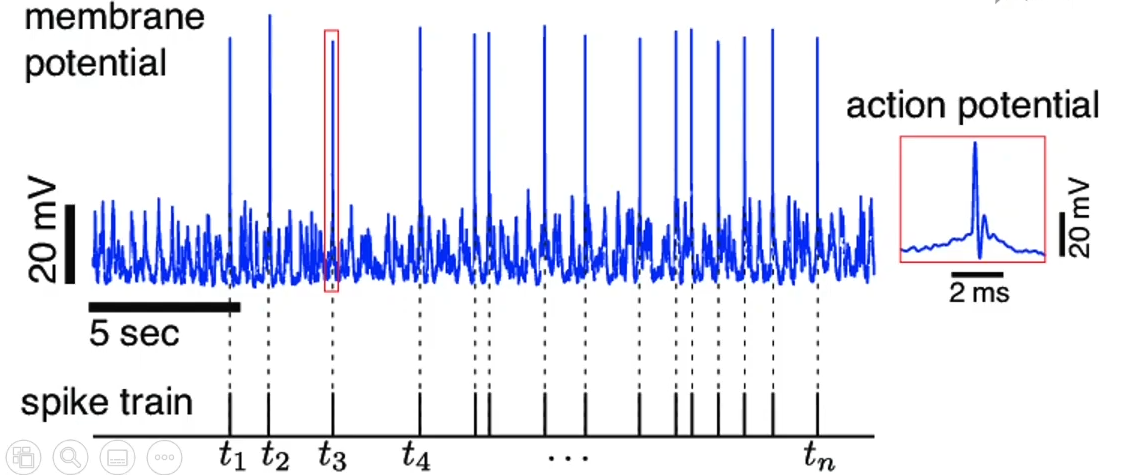
\includegraphics[width=0.7\linewidth]{images/neuronSpikes}
				\label{fig:neuronspike}
				\legend{Fonte: \cite{dan_goodman_2022_7044500}}
			\end{figure}
				
			\subsubsection{Neurônio de Pulso}
				\par Embora o foco deste trabalho seja nos \textit{Leaky Integrate and Fire Neurons} (LIF) porque são mais simples, mais eficientes e atualmente generalizam melhor para a maioria dos problemas \cite{dan_goodman_2022_7044500}.
		
		\subsubsection{Entendendo e modelando o LIF}
			
			\par O LIF é um dos modelos de neurônios mais simples em RNPs, ainda assim, pode ser aplicado com sucesso na maioria dos problemas em que as RNPs podem ser usadas, tal estrutura, assim como um neurônio de RN, recebe a soma das entradas ponderadas, mas, em vez de passá-lo diretamente para sua função de ativação, algum \textit{vazamento} é aplicado, diminuindo em algum grau o valor soma com o passar do tempo.
			
			\par O LIF se assemelha com circuitos Resistor-Capacitor, como pode ser visto na  \autoref{fig:rcmodel}. Aqui, $R$ é a resistência ao vazamento da corrente, $I_{in}$ é a corrente de entrada, $C$ é a capacitância, $U_{mem}$ representa é o potencial acumulado e $v$ é um interruptor que permite que o capacitor se descarregue (ou seja, emita um pulso) quando um determinado limiar de potencial é alcançado.
			
			\begin{figure}[h]
				\centering
				\caption[Modelo RC]{O modelo RC}
				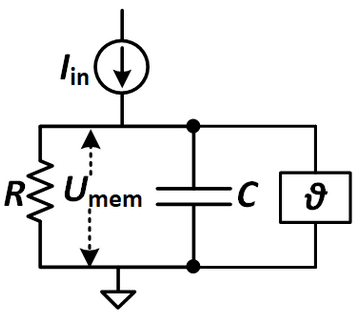
\includegraphics[width=0.3\linewidth]{images/rcmodel}
				\label{fig:rcmodel}
				\legend{Fonte: \cite{10242251}}
			\end{figure}
			
			\par Ao contrário do neurônio Hodgkin-Huxley, os pulsos são representados como \textbf{uns} dispersamente distribuídos em uma sequência de \textbf{zeros}, como ilustrado nas s \autoref{fig:pulsossparsitystaticsupress} e \autoref{fig:sparsity}. Essa abordagem simplifica os modelos e reduz a potência computacional e o armazenamento necessário para executar uma RNP.
			
			\begin{figure}[H]
				\centering
				\caption{Dispersão em Redes Neurais de Pulsos.}
				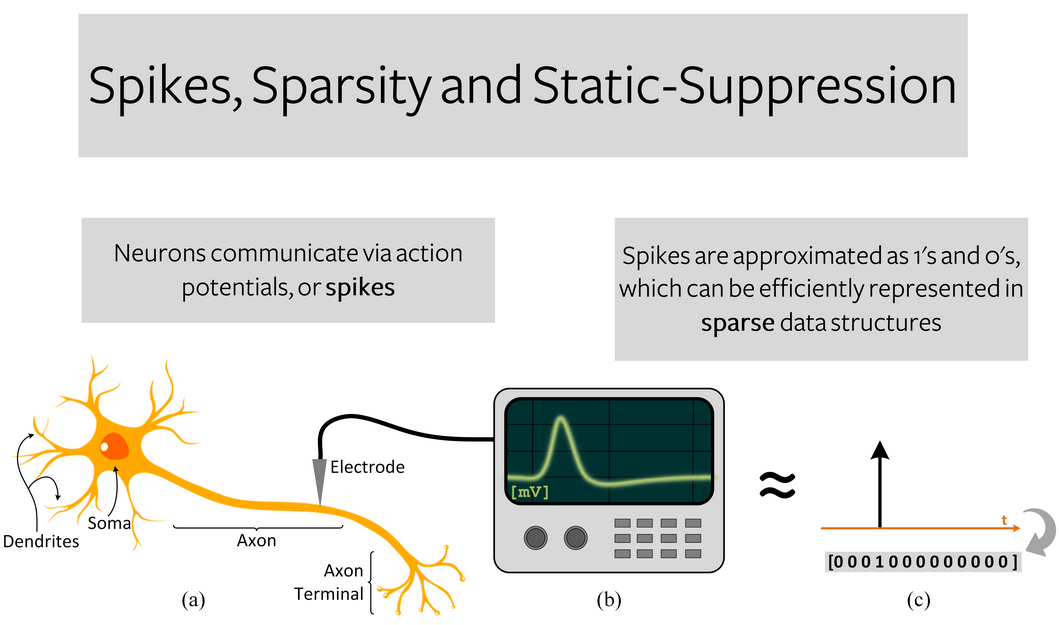
\includegraphics[width=.8\linewidth]{images/spikesSparsityStaticSupress}
				\legend{Fonte: \cite{10242251}}
				\label{fig:pulsossparsitystaticsupress}
			\end{figure}
			
			\begin{figure}[H]
				\centering
				\caption[Atividade dispersa de uma RNP]{Atividade dispersa de uma RNP: O eixo horizontal representa o momento no qual os dados estão sendo processados e o vertical representa o número do neurônio (índice) na RNP. Note que, na maior parte do tempo, muito poucos neurônios são ativados.}
				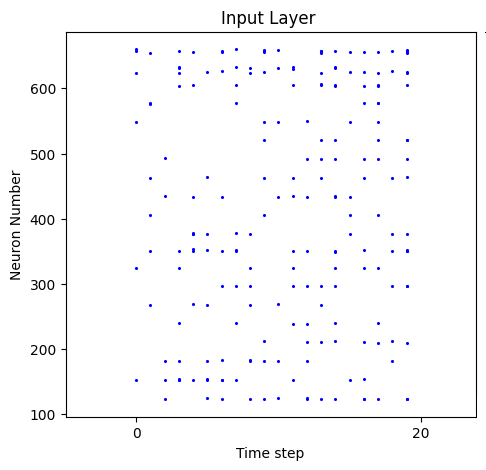
\includegraphics[width=.4\linewidth]{images/sparsity}
				\legend{Fonte: O autor.}
				\label{fig:sparsity}
			\end{figure}
						
			\par Como resultado do mencionado acima, em RNP, a informação é codificada no formato de \textit{tempo} e/ou \textit{taxa} de pulsos, proporcionando consequentemente grandes capacidades de processamento de fluxos de dados, mas limitando o processamento de dados estáticos.
			
			\par O modelo LIF é governado pelas equações abaixo \cite{10242251}.
			
			\par Considerando que $Q$ é uma medida de carga elétrica e $V_{\text{mem}}(t)$ é a diferença de potencial na membrana em um determinado tempo $t$, então a capacitância do neurônio $C$ é dada pela Equação \autoref{eq:capacitance}.
			
			\begin{equation}
				\label{eq:capacitance}
				C = \frac{Q}{V_{mem}(t)}
			\end{equation}
			
			\par Portanto, a carga do neurônio pode ser expressa pela \autoref{eq:charge}.
			
			\begin{equation}
				\label{eq:charge}
				Q = C.V_{mem}(t)
			\end{equation}
			
			\par Para saber como essa carga muda ao longo do tempo (ou seja, medir a corrente), podemos derivar $Q$ como na \autoref{eq:rateOfChargeChange}. Essa expressão representa a corrente na parte capacitiva do neurônio $I_C$.
			
			\begin{equation}
				\label{eq:rateOfChargeChange}
				I_C = \dfrac{dQ}{dt} = C. \dfrac{dV_{mem}(t)}{dt}
			\end{equation}
			
			\par Para calcular a corrente total passando pela parte resistiva do circuito, podemos usar a lei de Ohm:
			
			\begin{equation}
				\label{eq:ohmlaw}
				V_{mem}(t) = R.I_R \implies I_R = \frac{V_{mem}(t)}{R}
			\end{equation}
			
			\par Então, considerando que a corrente total não muda, como visto na  \autoref{fig:rcmodel2}, temos a corrente total de entrada $I_{in}$ do neurônio como na \autoref{eq:totalNeuronCurrent}.
			
			\begin{figure}[H]
				\centering
				\caption[Modelo RC para correntes]{Modelo RC para correntes: $I_{in} = I_R + I_C$}
				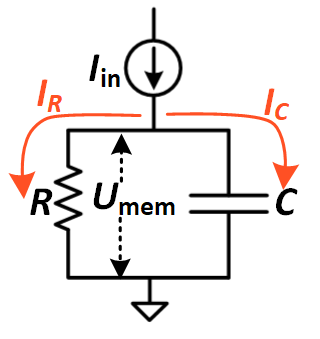
\includegraphics[width=0.3\linewidth]{images/rcmodel2}
				\legend{Fonte: \cite{10242251}}
				\label{fig:rcmodel2}
			\end{figure}
			
			\begin{equation}
				\label{eq:totalNeuronCurrent}
				I_{in}(t) = I_R + I_C \implies I_{in}(t) = \frac{V_{mem}(t)}{R} + C.\dfrac{dV_{mem}(t)}{dt}
			\end{equation}
		
			\par Portanto, para descrever a variação de potencial da membrana passiva, temos a \autoref{eq:memLinear}.
			
			\begin{equation}
				\label{eq:memLinear}
				\begin{aligned}
					I_{in}(t) &= \frac{V_{mem}(t)}{R} + C.\dfrac{dV_{mem}(t)}{dt} \implies \\ 
					I_{in}(t) - \frac{V_{mem}(t)}{R} &=  C.\dfrac{dV_{mem}(t)}{dt} \implies \\
					\Aboxed{R.I_{in}(t) - V_{mem}(t) &=  R.C.\dfrac{dV_{mem}(t)}{dt}}
				\end{aligned}
			\end{equation}
			
			\par Já que o no lado direito da equação $\left(\dfrac{dV_{mem}(t)}{dt}\right)$ expressa uma  grandeza em $voltagem/s$ e o esquerdo $\left(R.I_{in}(t) - V_{mem}(t)\right)$ em $voltagem$ apenas, conclui-se pela igualdade, que $R.C$ é uma unidade de tempo. Definindo $\tau = R.C$ como a \textbf{constante de tempo da membrana}, obtemos tensões em ambos os lados na \autoref{eq:finalMem}, que \textbf{descreve o circuito RC}.
			
			\begin{equation}
				\label{eq:finalMem}
				\begin{aligned}
					R.I_{in}(t) - V_{mem}(t) &=  R.C.\dfrac{dV_{mem}(t)}{dt} \implies \\
					R.I_{in}(t) - V_{mem}(t) &=  \tau.\dfrac{dV_{mem}(t)}{dt} \implies \\
					\Aboxed{\tau.\dfrac{dV_{mem}(t)}{dt} &= R.I_{in}(t) - V_{mem}(t)}
				\end{aligned}
			\end{equation}
			
			\par Então o comportamento do decaimento da voltagem no neurônio quando não há entrada $I_{in} = 0$ pode ser modelado, além disso, $R$ e $C$ não mudam e podem ser resumidos em $\tau = R.C$ que é uma constante. Portanto, atribuindo um potencial inicial $V_{mem}(0)$, se obtêm uma curva exponencial, como visto na \autoref{eq:expmembrane}.
			
			\begin{equation}
				\label{eq:expmembrane}
				\begin{aligned}
					\tau.\dfrac{dV_{mem}(t)}{dt} &= \cancel{R.I_{in}(t)} - V_{mem}(t) \implies \\
					\tau.\dfrac{dV_{mem}(t)}{dt} &= -V_{mem}(t) = \\
					\dfrac{dV_{mem}(t)}{dt} &= \dfrac{-V_{mem}(t)}{\tau} = \\
					\dfrac{dV_{mem}(t)}{V_{mem}(t)} &= \dfrac{-dt}{\tau} = \\
					\int\dfrac{1}{V_{mem}(t)}.dV_{mem}(t) &= \int\dfrac{-1}{\tau}.dt = \\
					\ln(|V_{mem}(t)|) &= -\dfrac{1}{\tau} . \int dt = \\
					\ln(|V_{mem}(t)|) &= -\dfrac{1}{\tau} . t = \\
					e^{\ln(|V_{mem}(t)|)} &= e^{-\frac{t}{\tau}} = \\
					V_{mem}(t) &= e^{-\frac{t}{\tau}} \implies \\
					\text{Considerando um valor inicial de } &V_{mem}(t) = V_{mem}(0) \text{ em } t=0 \implies \\
					\Aboxed{V_{mem}(t) &= V_{mem}(0).e^{-\frac{t}{\tau}}}
				\end{aligned}
			\end{equation}
			
			%TODO PARA CHEGAR NISSO
%			\par \textbf{PARA CHEGAR NISSO: } ${V_{mem}(t) = V_{mem}(0).e^{-\frac{t}{\tau}}}$ refazer considerando a constante c que a integral gera.
%			\begin{figure}[H]
%				\centering
%				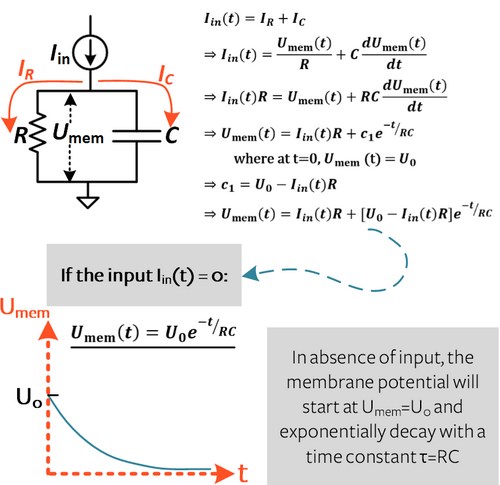
\includegraphics[width=0.7\linewidth]{apagar/screenshot001}
%				\caption{}
%				\label{fig:screenshot001}
%			\end{figure}
			
			
			\par Então, pode-se dizer que: Na ausência de uma entrada $I_{in}$, o potencial da membrana decai exponencialmente, como ilustrado na  \autoref{fig:membranepotentialdecay} e implementado no \autoref{lst:membranepotentialdecay}.
			
			\begin{lstlisting}[language=Python, caption={Python implementation of the action potential decaying of a LIF: $I_{in} = 0$}, label={lst:membranepotentialdecay}]
def lif(V_mem, dt=1, I_in=0, R=5, C=1):
	tau = R*C
	V_mem = V_mem + (dt/tau)*(-V_mem + I_in*R)
	return V_mem
\end{lstlisting}
			
			\begin{figure}[H]
				\centering
				\caption{Decaimento do potencial da membrana.}
				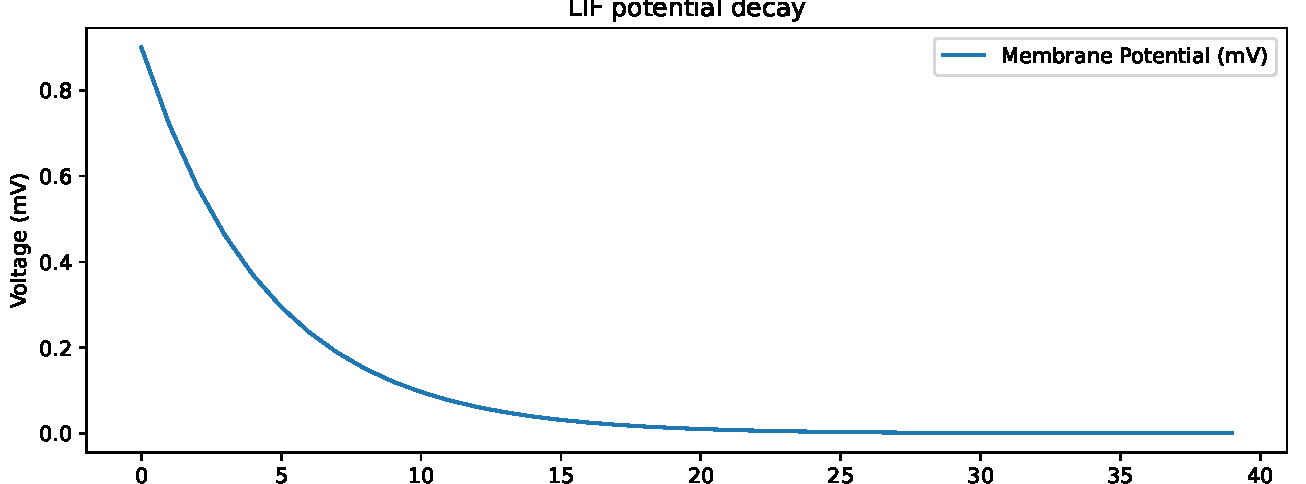
\includegraphics[width=.7\linewidth]{images/membranePotentialDecay}
				\legend{Fonte: O autor}
				\label{fig:membranepotentialdecay}
			\end{figure}
			
			\par Com os resultados da \autoref{eq:finalMem}, é possível calcular o aumento da voltagem, na presença de uma corrente de entrada, conforme visto na \autoref{eq:actionpotincrease0}.
			
			\begin{equation}
				\label{eq:actionpotincrease0}
				\begin{aligned}
					&\tau.\dfrac{dV_{mem}(t)}{dt} = R.I_{in}(t) - V_{mem}(t) = \\
					&\dfrac{dV_{mem}(t)}{dt} + \frac{V_{mem}(t)}{\tau} = \frac{R.I_{in}(t)}{\tau}
				\end{aligned}
			\end{equation}
			
			\par A \autoref{eq:actionpotincrease0} se encaixa na categoria de Equação Ordinária de primeira ordem, portanto, para resolvê-la se determina o fator de integração $f$ definido na \autoref{eq:actionpotincrease1}:
			
			\begin{equation}
				\label{eq:actionpotincrease1}
				\begin{aligned}
					f = e^{\int P(x) dx} \mid \dfrac{dy}{dx}&+P(x).y=Q(x) \therefore\\
					x &= t \\
					y &= V_{mem}(t) \\
					P(x) &= \frac{1}{\tau} \\
					Q(x) &= \frac{R.I_{in}}{\tau} \implies \\
					e^{\int \frac{1}{\tau} dx} &= e^{\frac{1}{\tau}.\int dt} = \boxed{e^{\frac{t}{\tau}}}
				\end{aligned}
			\end{equation}
			
			\par Fazendo a substituição do fator na \autoref{eq:actionpotincrease2}:
			
			\begin{equation}
				\label{eq:actionpotincrease2}
				\begin{aligned}
					\text{Substituindo em: } &(f.y)' = f.Q(x) \implies \\
					(e^{\frac{t}{\tau}}.V_{mem}(t))' &= \frac{R.I_{in}(t)}{\tau}.e^{\frac{t}{\tau}} \implies \\
					\int (e^{\frac{t}{\tau}}.V_{mem}(t))' &= \int \frac{R.I_{in}(t)}{\tau}.e^{\frac{t}{\tau}} dt \implies \\
					\Aboxed{e^{\frac{t}{\tau}}.V_{mem}(t) &= \frac{R.I_{in}(t)}{\tau}.\int e^{\frac{t}{\tau}} dt}
				\end{aligned}
			\end{equation}
			
			\par Que resolvendo pelo método da substituição na \autoref{eq:actionpotincrease3}:
			
			\begin{equation}
				\label{eq:actionpotincrease3}
				\begin{aligned}
					&u=\frac{t}{\tau} \implies \dfrac{du}{dt} = \dfrac{t}{\tau}dt \implies dt = du.\tau \therefore \\
					&\int e^u du.\tau = \tau.\int e^u du = \tau . e^u + c = \tau . e^{\frac{t}{\tau}} + c \implies \\
					&e^{\frac{t}{\tau}}.V_{mem}(t) = \frac{R.I_{in}(t)}{\tau}.\tau.e^{\frac{t}{\tau}} \implies \\
					&V_{mem}(t) = \frac{R.I_{in}(t)}{\tau . e^{\frac{t}{\tau}}}.\tau.e^{\frac{t}{\tau}} \implies \\
					& \text{Considering: } V_{mem}(t=0) = 0 \implies \\
					\Aboxed{&V_{mem}(t) = I_{in}(t).R(1-e^{\frac{1}{\tau}})}
				\end{aligned}
			\end{equation}
			
			
			\par Note que quando os potenciais de ação aumentam, ainda há um comportamento exponencial, como visto na  \autoref{fig:membranepotentialincrease} e implementado no  \autoref{lst:membranepotentialincrease}.
			
			\begin{lstlisting}[language=Python, caption={Python implementation of the action potential decreasing of a LIF: $I_{in}=1$}, label={lst:membranepotentialincrease}]
	
def lif(V_mem, dt=1, I_in=1, R=5, C=1):
	tau = R*C
	V_mem = V_mem + (dt/tau)*(-V_mem + I_in*R)
	return V_mem
\end{lstlisting}
			
			\begin{figure}[H]
				\centering
				\caption{Aumento do potencial da membrana.}
				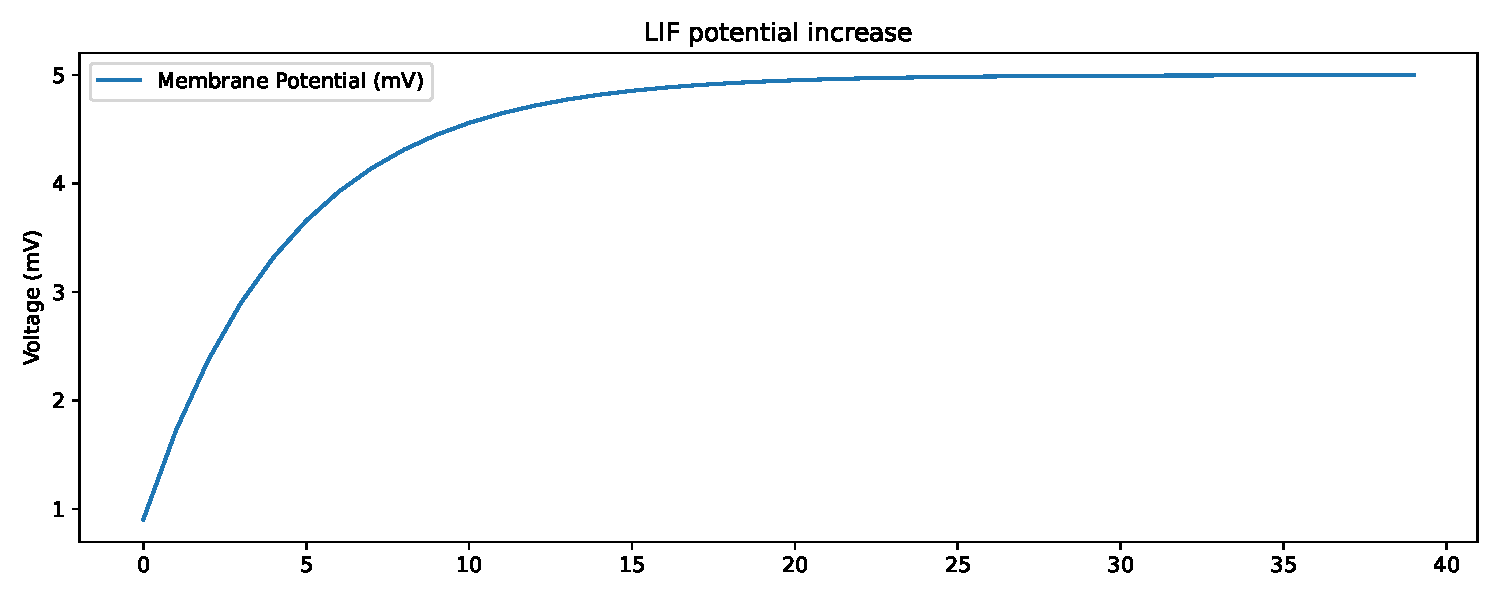
\includegraphics[width=.7\linewidth]{images/membranePotentialIncrease}
				\legend{Fonte: O autor}
				\label{fig:membranepotentialincrease}
			\end{figure}
			
			\par Levando em consideração um certo \textbf{limiar} que determina um \textit{reset} na voltagem do neurônio e dois tipos de \textit{resets} (para zero e subtração do limiar), finalmente é possível modelar o comportamento completo do LIF, conforme ilustrado na  \autoref{fig:membranepotentialfull} e implementado no \autoref{lst:membranepotentialfull}:
			
			\begin{lstlisting}[language=Python, caption={Python implementation of the action potential full simulation of a LIF: $I_{in}=1$, $V_{thresh} = 2$ is threshold}, label={lst:membranepotentialfull}]
def lif(V_mem, dt=1, I_in=1, R=5, C=1, V_thresh = 2, reset_zero = True):
	tau = R*C
	V_mem = V_mem + (dt/tau)*(-V_mem + I_in*R)
	if V_mem > V_thresh:
		if reset_zero:
			V_mem = 0
		else:
			V_mem = V_mem - V_thresh
	return V_mem
\end{lstlisting}

			
			\begin{figure}[H]
				\centering
				\caption[Gráfico do LIF]{Gráfico do LIF simulado completo: Foram fornecidos 0.5 mA de corrente no intervalo de tempo de 51 a 70.}
				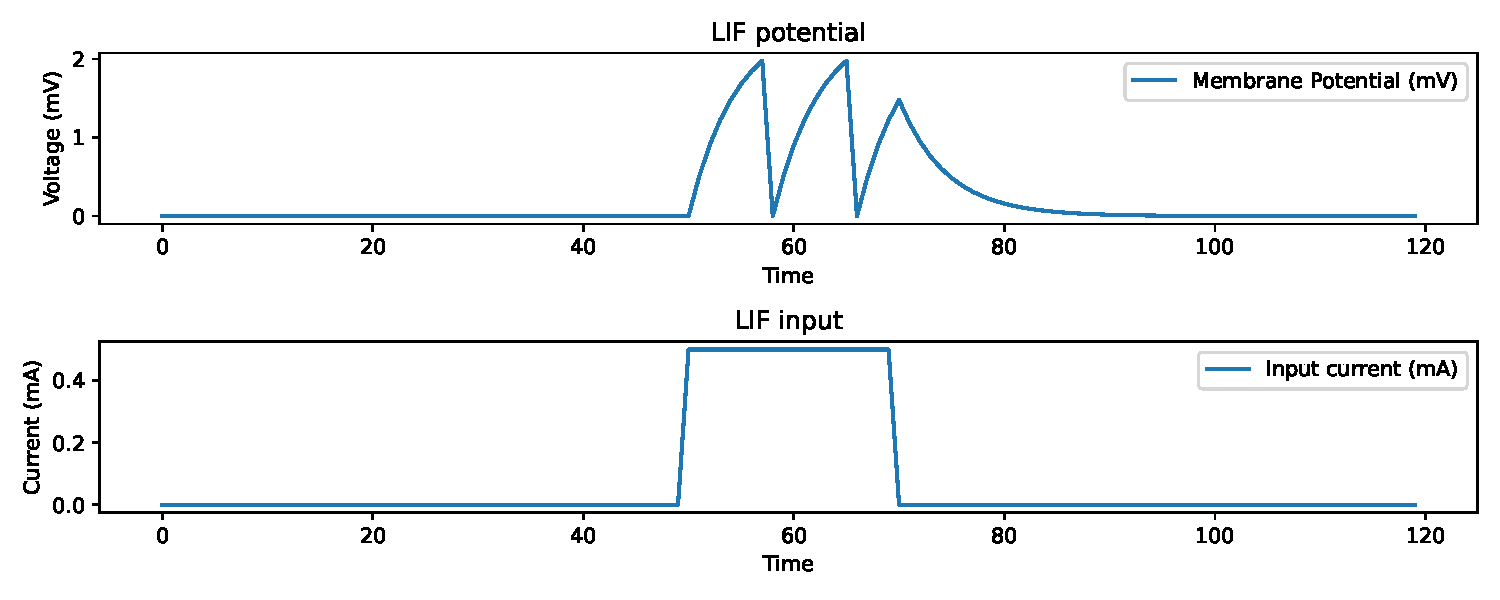
\includegraphics[width=.8\linewidth]{images/membranePotentialFull}
				\legend{Fonte: O Autor}
				\label{fig:membranepotentialfull}
			\end{figure}

			
		\subsubsection{Outra interpretação do LIF}
			
			\par Começando com a \autoref{eq:finalMem} e usando o Método de Euler para resolver o modelo LIF:
			
			\begin{equation}
				\tau.\dfrac{dV_{\text{mem}}(t)}{dt} = R.I_{\text{in}}(t) - V_{\text{mem}}(t)
			\end{equation}
			
			\par Resolvendo a derivada na \autoref{eq:membraneDerivative}, obtemos o potencial da membrana para qualquer tempo $t+\Delta t$ no futuro:
			
			\begin{equation}
				\label{eq:membraneDerivative}
				\begin{aligned}
					\tau.\dfrac{V_{\text{mem}}(t+\Delta t) - V_{\text{mem}}(t)}{\Delta t} &= R.I_{\text{in}}(t) - V_{\text{mem}}(t) = \\
					V_{\text{mem}}(t+\Delta t) - V_{\text{mem}}(t) &= \frac{\Delta t}{\tau} . (R.I_{\text{in}}(t) - V_{\text{mem}}(t)) = \\
					\Aboxed{V_{\text{mem}}(t+\Delta t) &= V_{\text{mem}}(t) + \frac{\Delta t}{\tau} . (R.I_{\text{in}}(t) - V_{\text{mem}}(t))}
				\end{aligned}
			\end{equation}

		\subsubsection{Treinamento}
		
			\par \textbf{Como as RNPs são treinadas?} Esta ainda é uma questão em aberto. Um neurônio RNP tem o comportamento de sua função de ativação mais parecido com uma \textbf{função de passo}. Portanto, em princípio, não podemos usar soluções baseadas em descida de gradiente porque esse tipo de função \textbf{não é} diferenciável \cite{kasabov2019time}.
			
			\par Mas existem algumas ideias que podem lançar alguma luz sobre este assunto: Enquanto algumas observações \textit{in vivo/in vitro} mostram que os cérebros, em geral, aprendem fortalecendo/enfraquecendo e adicionando/removendo sinapses, criando novos neurônios ou até mesmo outros métodos como pacotes de RNA. \cite{kasabov2019time} cita algumas outras formas:
			
			\begin{itemize}
				\item \textbf{Plasticidade Dependente do Tempo de Pulsos (STDP)}: Se um neurônio pré-sináptico dispara \textbf{antes} do pós-sináptico, há um fortalecimento na conexão, mas se o neurônio pós-sináptico disparar antes, então há um enfraquecimento.
				\item \textbf{Descida de Gradiente Emprestada}: Aproxima a função de passo usando outra função matemática, que é diferenciável (como uma sigmoide), para treinar a rede. Essas aproximações são usadas apenas na fase de \textit{backpropagation}, enquanto mantêm a função de passo na fase do \textit{feed-forward}.
				\item \textbf{Algoritmos Evolutivos}: Usam a seleção dos mais aptos ao longo de muitas gerações de redes.
				\item \textbf{Reservatório/Computação Dinâmica}: \textbf{Redes de estado de eco} ou \textbf{Máquinas de estado líquido}, respectivamente.
			\end{itemize}
		
		\subsection{\textit{Autoencoders}}
		
			\par Como ilustrado na  \autoref{fig:autoencoder} \textit{autoencoders} são redes neurais treinadas para reconstruir seus dados de entrada. Elas consistem em uma função codificadora, denotada como $h = f(x)$, e uma função decodificadora que produz uma reconstrução, denotada como $r = g(h)$. A camada oculta $h$ representa um \textbf{código} ou representação da entrada que pode ser ou não ser comprimida \cite{Goodfellow-et-al-2016}. Tais funções se traduzem em camadas como ilustrado na  \autoref{fig:autoencoder2} cujos neurônios são todos unidades ativas com ou sem funções de ativação. É importante destacar que um \textit{autoencoder} pode ser tão raso como o mostrado na \autoref{fig:autoencoder} ou $x$ e $r$ podem ser redes profundas.
			
			\par O principal objetivo de um \textit{autoencoder} é aprender uma representação dos dados de entrada na camada de \textbf{código} e, em seguida, reconstruir os dados de entrada com a maior precisão possível usando o decodificador. Geralmente, os \textit{autoencoders} são projetados para serem incapazes de copiar perfeitamente os dados de entrada pois isso os tornaria demasiadamente complexos e, em alguns casos, inúteis como será explicado adiante.

			\begin{figure}[h]
				\centering
				\caption[Representação funcional de um autoencoder]{Representação funcional de um \textit{autoencoder}: Sendo o vetor $x$ uma entrada, então o vetor $h$ é resultado da aplicação de uma função codificadora $f$ sobre $x$: $h = f(x)$, portanto $r$ é a reconstrução de $x$ a partir $h$ através de uma função decodificadora $g$: $r = g(h)$. Tal processo pode ou não implicar em uma perda de informação.}
				\begin{tikzpicture}[node distance=1.5cm, every edge/.style={draw=black,->}]
	% Nodes
	\node[draw, circle] (x) {$x$};
	\node[draw, rectangle, above right=0.7cm and 1cm of x] (encoder) {Codificador};
	\node[draw, circle, above right=0.7cm and 1cm of encoder] (h) {$h$};
	\node[draw, rectangle, below right=0.7cm and 1cm of h] (decoder) {Decodificador};
	\node[draw, circle, below right=0.7cm and 1cm of decoder] (r) {$r$};
	
	% Arrows
	\draw (x) edge (encoder);
	\draw (encoder) edge (h);
	\draw (h) edge (decoder);
	\draw (decoder) edge (r);
	
	% Loss
	\node[below of=h, yshift=-0.7cm] (loss) {Perda na reconstrução};
	\draw (x) edge (loss);
	\draw (r) edge (loss);
	
	% Labels
	\node[below of=x, yshift=0.7cm] {Entrada};
	\node[below right=0.2cm and 0.8cm of decoder] {Saída};
	\node[below of=r, yshift=0.7cm] {Entrada reconstruida};
\end{tikzpicture}
				\legend{Fonte: O Autor}
				\label{fig:autoencoder}
			\end{figure}
		
			\par Considerando-se que a reconstrução $r$ seja razoável, isso significa que a região $h$  contém dados suficientes para representar a informação em sua essência, sendo assim, \textit{autoencoders} são ótimos produtores de vetores de características. Hipoteticamente é possível criar \textit{autoencoders} cuja a camada de código seja apenas um número inteiro caso tanto o codificador quanto o decodificador sejam grandes e complexos o suficiente, mas isso se mostraria inútil caso se necessitasse algum tipo de representação da informação original que fosse significativa, ademais, excluindo-se casos triviais, segundo \cite{Goodfellow-et-al-2016} isso ainda não se verifica na prática.

			\begin{figure}[h]
				\centering
				\caption[Exemplo esquemático de um autoencoder]{Exemplo esquemático de um \textit{autoencoder}: Os nós de entrada estão em cinza, a camada de código em amarelo contêm as características codificadas e finalmente a camada de reconstrução em vermelho contêm um cópia aproximada da entrada.}
				\begin{tikzpicture}[scale=2.5]
	% Define scaling factors
	\def\inputscale{.5}
	\def\hiddenscale{.5}
	\def\outputscale{.5}
	
	%input layer
	\foreach \i in {0,1,2,3,4} {
		\node (input_node\i) at (0,\i*\inputscale) {}; 
		\filldraw[fill=gray] (input_node\i) circle (0.15cm);
		\node at (input_node\i) {\tiny $x_\i$};
		
		\draw[->,in=180,out=0] (-0.5,\i*\inputscale) to (input_node\i);
	}
	
	%hidden layer
	\foreach \i in {0,1,2} {
		\node (hidden_node\i) at (1.5,\i*\hiddenscale+.5) {}; 
		\filldraw[fill=yellow] (hidden_node\i) circle (0.15cm);
		\node at (hidden_node\i) {\tiny $h_\i$};
	}
	
	%output layer
	\foreach \i in {0,1,2,3,4} {
		\node (output_node\i) at (3,\i*\outputscale) {}; 
		\filldraw[fill=red] (output_node\i) circle (0.15cm);
		\node at (output_node\i) {\tiny $r_\i$};
	}
	
	% Connect layers
	\foreach \i in {0,1,2,3,4} {
		\foreach \j in {0,1,2} {
			\draw[->,in=180,out=0] (input_node\i) to (hidden_node\j);
			\draw[->,in=180,out=0] (hidden_node\j) to (output_node\i);
		}
	}
	
	%descriptions
	\draw[snake=brace,mirror snake,raise snake=45pt,brown] (-0.2,0.4) -- (0.3,0.4) node[black,midway,yshift=-50pt,below]{\tiny entrada};
	
	\draw[snake=brace,mirror snake,raise snake=45pt,brown] (1.3,0.8) -- (1.7,0.8) node[black,midway,yshift=-50pt,below]{\tiny código};
	
	\draw[snake=brace,mirror snake,raise snake=45pt,brown] (2.7,0.4) -- (3.3,0.4) node[black,midway,yshift=-50pt,below]{\tiny reconstrução};

\end{tikzpicture}
				\legend{Fonte: O Autor}
				\label{fig:autoencoder2}
			\end{figure}

			\par Em se tratando de treinamento as técnicas já conhecidas e testadas para redes neurais em geral (como, por exemplo, \textit{gradient descent} com \textit{minibatch} ou estocástico) podem ser usadas  \cite{Goodfellow-et-al-2016} incluindo as formas de regularização com será exposto mais adiante.
			
			\subsubsection{Autoencoders sub-completos ou clássicos}
				\par Esse tipo de rede neural, como ilustrado na  \autoref{fig:autoencoder2}, tem sua camada de código limitada em dimensionalidade para apenas aproximar a entrada e priorizar certos aspectos dos dados extraindo dessa forma os componentes mais cruciais e significativos de um conjunto de dados \cite{Goodfellow-et-al-2016}. Um autoencoder clássico age de forma muito semelhante ao algoritmo
				\textit{Principal Component Analysis} (PCA) \cite{bengio2014representation}.
				  
			\subsubsection{Autoencoders supra-completos}
			
				\begin{figure}[H]
					\centering
					\caption[Exemplo esquemático de um autoencoder supra-completo]{Exemplo esquemático de um \textit{autoencoder} supra-completo.}
					\begin{tikzpicture}[scale=2.5]
	% Define scaling factors
	\def\inputscale{.5}
	\def\hiddenscale{.5}
	\def\outputscale{.5}
	
	%input layer
	\foreach \i in {0,1,2} {
		\node (input_node\i) at (0,\i*\inputscale) {}; 
		\filldraw[fill=gray] (input_node\i) circle (0.15cm);
		\node at (input_node\i) {\tiny $x_\i$};
		
		\draw[->,in=180,out=0] (-0.5,\i*\inputscale) to (input_node\i);
	}
	
	%hidden layer
	\foreach \i in {0,1,2,3,4} {
		\node (hidden_node\i) at (1.5,\i*\hiddenscale-0.65) {}; 
		\filldraw[fill=yellow] (hidden_node\i) circle (0.15cm);
		\node at (hidden_node\i) {\tiny $h_\i$};
	}
	
	%output layer
	\foreach \i in {0,1,2} {
		\node (output_node\i) at (3,\i*\outputscale) {}; 
		\filldraw[fill=red] (output_node\i) circle (0.15cm);
		\node at (output_node\i) {\tiny $r_\i$};
	}
	
	% Connect layers
	\foreach \i in {0,1,2} {
		\foreach \j in {0,1,2,3,4} {
			\draw[->,in=180,out=0] (input_node\i) to (hidden_node\j);
			\draw[->,in=180,out=0] (hidden_node\j) to (output_node\i);
		}
	}
	
	%descriptions
	\draw[snake=brace,mirror snake,raise snake=45pt,brown] (-0.2,0.4) -- (0.3,0.4) node[black,midway,yshift=-50pt,below]{\tiny entrada};
	
	\draw[snake=brace,mirror snake,raise snake=45pt,brown] (1.3,-0.2) -- (1.7,-0.2) node[black,midway,yshift=-50pt,below]{\tiny código};
	
	\draw[snake=brace,mirror snake,raise snake=45pt,brown] (2.7,0.4) -- (3.3,0.4) node[black,midway,yshift=-50pt,below]{\tiny reconstrução};
	
\end{tikzpicture}
					\legend{Fonte: O Autor}
					\label{fig:autoencoder3}
				\end{figure}
			
				\par Como mostrado na  \autoref{fig:autoencoder3}, ao contrário dos autoencoders sub-completos, os supra-completos tem sua camada de código com uma \textbf{dimensão maior} do que os dados de entrada. Dessa forma as características dos dados de entrada podem ser codificadas mais de uma vez e uma reconstrução perfeita é atingida. Estruturas assim são inúteis já que não conseguem extrair características significativas a não ser que sejam aplicadas técnicas de regularização \cite{bengio2014representation}.
				
			\subsubsection{\textit{Autoencoders} regularizados}
				
				\par Segundo \cite{bengio2014representation} uma das formas de regularização é justamente a limitação da dimensão da camada de código, a mesma aplicada aos \textit{autoencoders} sub-completos, como estes já foram explicados apresentar-se-ão a seguir outras formas de regularização.
				
				\par Considerando que \textit{autoencoders} devem ser treinados para minimizar uma função de erro $E$ que compara a entrada original $x$ com a reconstrução $r$ então um autoencoder \textbf{regularizado} deve ter adicionado a essa função um termo de regularizador $\phi$ como a mostrado na \autoref{eq:autoreg} que é um termo que pode corresponder a uma regularização L1, L2, $\Omega(h)$ (discutidas no apêndice \autoref{Apend:regularization}).
				
				\begin{equation}
					\label{eq:autoreg}
					E(x, r) + \phi
				\end{equation}
			
				\par Segundo \cite{Goodfellow-et-al-2016} usando técnicas de regularização é possível até mesmo para um \textit{autoencoder} supra-completo que o mesmo extraia características úteis para uso. Tais técnicas devem prover a seguintes propriedades para a rede:
				
				\begin{itemize}
					\item dispersão: É a tendência de ativar apenas um pequena quantidade das unidades (também conhecidas como dimensões) da camada de código para qualquer entrada dada criando uma representação mais compacta.
					\item pequena variação no gradiente: Garantir pouca amplitude nos valores dos gradientes em relação as variações ou ruídos de uma entrada evita que grandes flutuações ocorram na camada de código proporcionando um comportamento estável.
				\end{itemize}

				
			\subsubsection{\textit{Denoising autoencoders}}
				\par Tais redes também podem ser caracterizadas como \textit{autoencoders} regularizados. Porém há diferenças: Aqui o foco não é criar funções de regularização e sim adicionar ruídos \textbf{apenas} na informação de entrada mas mantendo a intactos os dados que serão comparados na função de erro como mostra a  \autoref{fig:denoisingAutoencoder}. Um \textit{autoencoder} treinado dessa forma, além de ser mais resiliente a ruídos, também adquirire uma funcionalidade de preencher falhas de informação nos dados de entrada quando o componente adicionador de ruído é removido e os dados são diretamente apresentados a rede.
				
				\begin{figure}[h]
					\centering
					\caption[Representação funcional de um \textit{denoising autoencoder}]{Representação funcional de um \textit{denoising autoencoder}: Sendo o vetor $x$ uma entrada e $n$ um função que adiciona um ruído aleatório então a informação com ruído $\hat{x}$ é definida como $\hat{x} = n(x)$, portanto o vetor $h$ é resultado da aplicação de uma função codificadora $f$ sobre $x$: $h = f(x)$, finalmente $r$ é a reconstrução de $x$ a partir $h$ através de uma função decodificadora $g$: $r = g(h)$. É importante notar que $r$ é comparada com $x$ e não com $\hat{x}$.}
					\begin{tikzpicture}[node distance=3cm, every edge/.style={draw=black,->}]
	% Nodes
	\node[draw, rectangle, fill=blue] (x) {$x$};
	
	\node[draw, rectangle, above right=-.6cm and 1cm of x] (noiser) {$n(x)$};
	
	\node[draw, circle, above right=-.6cm and 1cm of noiser, fill=gray] (x_hat) {$\hat{x}$};
	
	\node[draw, rectangle, above right=0.7cm and 1cm of x_hat] (encoder) {$f(\hat{x})$};
	
	\node[draw, circle, above right=0.7cm and 1cm of encoder, fill=yellow] (h) {$h$};
	
	\node[draw, rectangle, below right=0.7cm and 1cm of h] (decoder) {g(h)};
	
	\node[draw, circle, below right=0.7cm and 1cm of decoder, fill=red] (r) {$r$};
	
	% Arrows
	\draw (x) edge (noiser);
	\draw (noiser) edge (x_hat);
	\draw (x_hat) edge (encoder);
	\draw (encoder) edge (h);
	\draw (h) edge (decoder);
	\draw (decoder) edge (r);
	
	% Loss
	\node[below of=h, yshift=-0.7cm] (loss) {eventual perda na reconstrução};
	\draw [->,in=180,out=-90](x) edge (loss);
	\draw [->,in=0,out=-90] (r) edge (loss);
	
	% Labels
	\node[above of=x, yshift=-2cm] {entrada};
	\node[above of=r, yshift=-2cm, xshift=.5cm] {reconstrução};
\end{tikzpicture}
					\legend{Fonte: O autor}
					\label{fig:denoisingAutoencoder}
				\end{figure}
							
		\subsection{Redes neurais residuais (ResNets)}
			\par Segundo \cite{DBLP:journals/corr/HeZRS15} a ideia-chave por trás das \textit{ResNets} é a inclusão de conexões de salto como ilustrado na  \autoref{fig:residualblock}, também conhecidas como mapeamentos de identidade, permitindo que a saída de uma camada seja adicionada elemento-a-elemento diretamente à entrada de uma camada subsequente. Para que isso aconteça é importante que tanto a saída quanto a entrada tenham a mesma dimensão.
			
			\begin{figure}[H]
				\centering
				\caption[Bloco residual]{Bloco Residual: $x$ contorna as camada intermediárias $F(x)$ via uma função identidade somando-se a $F(x)$ ao final do bloco.}
				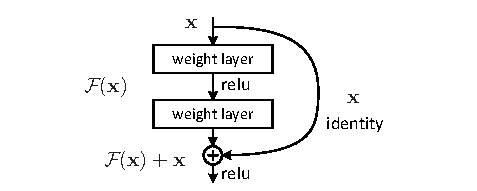
\includegraphics[width=0.7\linewidth]{images/residualBlock}
				\legend{Fonte: \cite{DBLP:journals/corr/HeZRS15}}
				\label{fig:residualblock}
			\end{figure}
			
			
			\par Quando uma rede chega a um certo limite de acurácia, intuitivamente se pode pensar que adicionando mais camadas o desempenho da mesma melhore, no entanto, na prática isso não se verifica. O que se observa em redes mais profundas pode ser exatamente o contrário como mostrado na \autoref{fig:teaser}.
			
			\begin{figure}[H]
				\centering
				\caption[Comparação de redes profundas não residuais]{Desempenho de duas redes neurais não residuais com 56 e 20 camadas. A esquerda a taxa de erro durante o treinamento, a direita a taxa de erro em relação ao conjunto de testes.}
				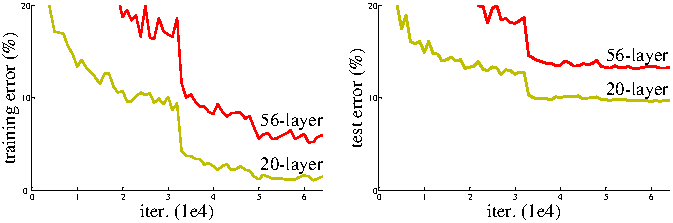
\includegraphics[width=0.7\linewidth]{images/teaser}
				\legend{Fonte: \cite{DBLP:journals/corr/HeZRS15}}
				\label{fig:teaser}
			\end{figure}
			
			\par Redes neurais muito profundas podem sofrer de problemas como o desaparecimento ou explosão do gradiente, onde os gradientes (ou seja, as direções para ajustar os pesos da rede) se tornam muito pequenos ou grandes à medida que são retro-propagados durante o treinamento. Isso pode dificultar o treinamento eficaz das camadas mais profundas.

			\par Então já que, empiricamente, as redes com menos camadas estão expostas a menos problemas de otimização, se pode juntar várias dessas formando assim uma rede mais profunda e com mais hiperparâmetros que podem ser ajustados. Isso, aliado as técnicas de regularização diminui a ocorrência do desaparecimento ou explosão de gradientes, um problema comum em redes com muitas camadas que pode piorar, impossibilitar ou diminuir a níveis impraticáveis o aprendizado da rede \cite{DBLP:journals/corr/HeZRS15}. 
			
			\par Em vez de aprender a mapear diretamente de $x$ para $y$, as camadas da rede aprendem a mapear de $x$ para a diferença entre $x$ e $y$, ou seja, para o \textbf{resíduo}. Isso simplifica o treinamento, pois a rede precisa apenas ajustar os resíduos, em vez de aprender a mapear completamente as entradas para as saídas.
			
			\par Além das características já expostas as redes residuais não adicionam complexidade computacional além da negligenciável adição elemento-a-elemento. Isso facilita a comparação com redes não residuais com o mesmo número de hiperparâmetros.
			
			\subsubsection{Aprendizado residual}
			
				\par Considerando então $x$ como a entrada de uma rede, $f(\cdot)$ como uma série de camadas cujas sucessivas aproximações, via treinamento, resultam em um desejado  estado intermediário na camada escondida $h$, então o que se convenciona chamar de resíduo $r$ é dado na \autoref{eq:residuo} considerando que $h$ e $x$ tenha a mesma dimensão.
				
				
				\begin{equation}
					\label{eq:residuo}
					r = h - x
				\end{equation}
			
				\par Considerando o resíduo, então se pode reformular o estado $h$ como mostrado na \autoref{eq:residuoH} demonstrando que, para se mapear $x$ em $h$ basta que $f(\cdot)$ atue sobre $r$, ou seja, que as aproximações sucessivas sejam feitas sobre o resíduo $r$.
				
				\begin{equation}
					\label{eq:residuoH}
					h = r + x
				\end{equation}
			
				\par Se em uma rede não profunda forem adicionadas camadas cuja a única função é receber uma entrada e devolvê-la sem modificações (função identidade) então é trivial que uma rede possa atingir grandes profundidades. No entanto segundo \cite{DBLP:journals/corr/HeZRS15} em redes profundas os otimizadores tem dificuldade em aprender tais funções identidade levando a degradação do desempenho como mostrado na \autoref{fig:teaser}. Nas redes residuais se os mapeamentos identidade (também chamados de conexões de atalho) forem ótimos os otimizadores podem simplesmente zerar todos os pesos das camadas intermediárias de um bloco residual.
				

				\begin{figure}[h]
					\centering
					\caption[Obtenção do resíduo]{Obtenção do resíduo: $x$ um vetor de entrada na rede, $I(\cdot)$ é uma função identidade cujo valor é diretamente somado $\oplus$ com o resultado produzido pelas várias camadas representadas por $f(\cdot)$, $h$ é um vetor representando um estado intermediário de uma rede neural.}
					\begin{tikzpicture}[node distance=3cm, every edge/.style={draw=black,->}]
	% Nodes
	\node[draw, rectangle, fill=blue] (x) {$x$};
	\node[draw, rectangle, above right=-.6cm and 1cm of x] (function) {$r = f(x)$};
	\node[draw, rectangle, above right=1cm and -1.1cm of function] (identi) {$I(x)$};
	\node[draw, circle, above right=-.5cm and 4cm of x] (plus) {$+$};
	\node[draw, rectangle, above right=-.6cm and 1.5cm of plus, fill=gray] (hidden) {$h$};
	
	% Arrows
	\draw (x) edge (function);
	\draw (function) edge (plus);
	\draw (plus) edge (hidden);
	
	
	\draw [->,in=180,out=90](x) edge (identi);
	\draw [->,in=90,out=0] (identi) edge (plus);
	

	% Labels
	\node[above of=identi, yshift=-2.4cm] {Identidade};
	\node[above of=x, yshift=-4cm] {Entrada};
	\node[above of=hidden, yshift=-4cm, xshift=0cm] {Estado intermediário};
\end{tikzpicture}
					\legend{Fonte: O autor}
					\label{fig:residuo}
				\end{figure}
			
				\par O bloco residual mostrado na \autoref{fig:residuo} torna mais fácil para a rede se aproximar de funções identidade pois basta a mesma zerar os pesos constituintes das camadas representadas por $f(\cdot)$. Note que $f(\cdot)$ é flexível e portanto pode ter $n$ camadas constituintes e que essa estrutura pode ser usada multiplas vezes sozinha ou em conjunto com outras estruturas em uma rede.

	\section{Trabalhos mais recentes}
	
		\par Afim de entender melhor o campo de pesquisa, além de formar uma boa base para compreensão do assunto, foram levantados os métodos de autenticação por fala e/ou análise de sinais cerebrais. A coleta dos trabalhos foi feita segundo os parâmetros descritos a seguir.
		
		\subsection{Protocolo de coleta}
		
			\par \textbf{Critérios de inclusão e exclusão} de artigos:
			\begin{itemize}
				\item dos últimos 5 anos
				\item que correspondiam às palavras-chave de pesquisa constantes na \autoref{tab:basesdedados}
				\item cujo \textit{abstract} continha as bases de dados usadas, os resultados e a metodologia brevemente descritos.
			\end{itemize}
			
			
			\par A \textbf{estratégia de busca} dos artigos foi guiada segundo a base de dados e palavras-chaves constantes na \autoref{tab:basesdedados}.
			\begin{table}[H]
				\begin{center}
					\caption[Bases de dados usadas]{Bases de dados usadas}
					\begin{tabular}{|l|l|l|l|}
						\hline
						Base de dados & Palavras chave & Filtros aplicados & Limitações \\
						\hline
						Web of Science & & & \\
						\hline
						ACM & & & \\
						\hline
						Elsevier & & & \\
						\hline
						IEEE & & & \\
						\hline
					\end{tabular}
					\label{tab:basesdedados}
					\legend{Fonte: Elaborado pelo autor, 2024}
				\end{center}
			\end{table}
		
			\par O primeiro estudo consultado \cite{ParkHyeong-jun2023Mcoi} aborda o uso de EEG para captação de fala imaginada usando as técnicas de decomposição de sinal NA-MEMD (\textit{multivariate empirical mode decomposition}) e DTWPT (Discrete time Wavelet Package Transform) e a arquitetura de redes neurais MRF-CNN. A NA-MEMD é uma extensão do EMD (\textit{Empirical mode decomposition}) para sinais multivariados permitindo a decomposição de sinais. O MRF-CNN é uma arquitetura de rede neural convolucional profunda que utiliza características estatísticas extraídas dos sinais decompostos como entrada para o classificador. Foram utilizadas técnicas de validação cruzada e divisão de dados para treinamento e teste do classificador. Os dados EEG foram coletados dos nove participantes saudáveis, estes tiveram que imaginar as vogais "a", "e", "i", "o", "u". O estudo atingiu uma média de 80,41\% de classificações corretas.
			
			\par Em \cite{AbdulghaniMokhlesM2023ISCU} usa \textit{Wavelet Scattering Transform} (WST), técnica que aplica sobre o sinal transformadas wavelet combinadas com operações não lineares, para extração de características para posterior classificação por uma Rede Neural LSTM(\textit{Long-Short term memory}) recorrente. Os quatro participantes imaginaram as seguintes expressões: \textit{"up", "down", "left" e "right"}. Em testes a acurácia alcançada foi 92,50\%.
			
			\par Com o fim de remover ruídos e artefatos causados por movimentos musculares relacionados a região da cabeça em \cite{MahapatraNrushinghCharan2023Ecoi} foi usada a DTWT (\textit{Discrete Time Wavelet Transform}) para processar os sinais EEG, que foram obtidos a partir das bases de dados EPOC e MUSES \cite{mindbigdata}. Depois da filtragem e geração de características variações de Redes Neurais Recorrentes Bidirecionais foram empregadas na classificação das classes compostas pelos dígitos de 0 a 9. Foram alcançadas acurácias máximas de 98,18\% na base MUSE e 71,60\% na EPOC.
			
			\par Nesta revisão \cite{ShahUzair2022TRoA} que foi feita segundo as orientações constantes no protocolo PRISMA-ScR foram selecionados 34 trabalhos que analisaram palavras e expressões imaginadas, nestes, a técnica mais usada para extração de características foram os filtros Wavelet e os algoritmos de classificação mais proeminentes foram as \textit{Support Vector Machines}(SVM) e as Redes Neurais Convolucionais. É reportado os estudos utilizam poucos tipos de métricas limitando-se na maioria dos casos a acurácia, a revisão sugere que também sejam usadas métricas como: Precisão, \textit{Recall}, Taxa de erro de palavras (Word Error Rate), AUC (Área Under the Curve), Sensitividade, Especificidade e Média Quadrática afim de se oferecer uma visão mais geral dos resultados. 
			
			\par Uma combinação de redes neurais convolucionais temporais (TCN) e convolucionais tradicionais (CNN) foi usada no estudo \cite{MahapatraNrushinghCharan2022MCoI} para classificar sinais de EEG pré-processados pelo algoritmo de Análise Independente de Componentes (\textit{FastICA}) afim de proporcionar uma melhor separação dos canais e por DTWT para remoção de artefatos e criação dos vetores de características. Os sinais foram obtidos da base \cite{10.1117/12.2255697} que é composta por sinais produzidos por 15 indivíduos falantes de espanhol com as vogais "a", "e", "i", "o", "u" e com os comandos \textit{"arriba", "abajo", "derecha" e "isquierda"}. O estudo alcançou uma acurácia de 96,49\%.

			\par Para classificar as letras do alfabeto imaginadas em inglês por 13 indivíduos o estudo \cite{AgarwalPrabhakar2022Ebia} usou a DTWT para remoção ruídos e separação de bandas de frequência do sinal a ser classificado por dois algoritmos simultaneamente: Árvores Aleatórias (ou \textit{Random Forrest})(RF) e SVM. O estudo alcançou uma acurácia média entre as classificações de todos os elementos do alfabeto de 77,97\%. Neste trabalho também foi utilizado o método \textit{Common Average Referecing}(CAR) que, via a subtração de uma média dos sinais captados em um certo intervalo de tempo, procura remover interferências induzidas em todos os eletrodos por variáveis ambientais aumentando a relação sinal/interferência (\textit{Signal-to-noise ratio})(SNR). Uma interessante constatação desse trabalho é de que as ondas cerebrais $\alpha$, $\beta$ e $\theta$ quando consideradas sozinhas melhoram o desempenho dos classificadores.
			
			\par Aqui \cite{Hernandez-Del-ToroTonatiuh2021TaEB} usa os seguintes métodos de extração de características: DTWT (para obtenção da energia de bandas), EMD, dimensões fractais e características extraídas segundo metodos da teoria do caos. Os dados foram obtidos a fim de se criar 3 bases de dados contendo as palavras em espanhol \textit{"arriba", "abajo", "derecha" e "isquierda"}, a primeira continha informações de 27 pessoas, a segunda também 27 e a terceira 20. Na primeira e segunda bases a taxa de captura foi de 128Hz e na terceira 500Hz, esta foi subamostrada para 128Hz a posteriori. Para remoção de ruído o método CAR foi usado. Os classificadores usados foram RF, \textit{K-nearest-neighbors}(KNN), SVM e Regressão Logística. Para avaliação as métricas Pontuação F1 (PF1), Precisão e \textit{Recall} foram usadas. Os melhores resultados obtidos nas bases 1, 2 e 3 foram respectivamente: 0,73, 0,79 e 0,68 para PF1, 0,66, 0,70, 0.65 para Precisão e 0,87, 0,93 e 0,83 para \textit{Recall}.
			
			\par Constante nas referências de \cite{Hernandez-Del-ToroTonatiuh2021TaEB} um dos poucos trabalhos que discorreram sobre a identificação de pessoas \cite{MOCTEZUMA2019201} usou CAR para melhorar a SNR dos sinais armazenados e amostrados a 128Hz correspondentes as palavras em espanhol \textit{"arriba", "abajo", "derecha" e "isquierda"} imaginadas por 27 voluntários. A geração do vetor de características foi feita usando DTWT em 4 níveis e para cada nível foi calculada a Energia de \textit{Teager} ou \textit{Teager Energy Operator} (TEO). RF foi usada como classificador. Os resultados variaram entre 85\% quando todos os 27 indivíduos foram incluídos até 97\% quando apenas 5 foram considerados.
			
			\par Dada a pouca quantidade de dados e bases existentes quando se trata de EEG, o artigo \cite{PanachakelJerrinRamakrishnan} usou uma técnica de expansão de informação baseada em "janelas deslizantes" ao mesmo tempo em que, em vez de considerar separadamente cada sensor, agrupou os dados dos mesmos em matrizes tridimensionais semelhantes a imagens que foram processadas por uma rede Resnet50 \cite{DBLP:journals/corr/HeZRS15} adaptada usando a técnica de transferência de aprendizado. A base de dados usada \cite{nguyen2018inferring} é composta por EEG capturado de 64 canais a 1000Hz para as seguintes falas imaginadas por 11 pessoas do sexo masculino e 4 do feminino: \textit{"independent", "cooperate", "in", "out", "up", "a", "i", "u"}. As taxas de amostragem foram posteriormente diminuídas para 250Hz e filtradas para remoção de ruídos e artefatos. Os resultados variaram de um mínimo de 79,7\% de acurácia para classificação de vogais até um máximo de 95,5\% para palavra curtas e longas.
			
			\par \cite{tamm2020classification} usou uma base de dados composta por 15 voluntários imaginando as letras \textit{"a", "e", "i", "o", "u"} e mais seis diferentes palavras \cite{10.1117/12.2255697} e simplificou a estrutura de uma CNN criada em outro estudo usando uma técnica de transferência de aprendizado enquanto tentou manter a mesma acurácia. Os dados iniciais foram submetidos a sub-amostragem para que se chegasse a uma taxa de amostragem de 128Hz e dispostos em uma matriz de duas dimensões. O classificador simplificado atingiu uma acurácia média de 23,98\%.
			
			\par \cite{Panachakel_2019} utilizou 11 palavras da base de dados \cite{7178118}, extraindo de cada canal características baseadas em transformadas \textit{Wavelet} de nível 7, alcançando uma acurácia média de 57,15\%. A inovação aqui foi tratar separadamente os vetores de características dos 11 canais, inserindo-os, um por vez, em uma rede neural profunda com 2 camadas ocultas. A classificação foi realizada por votação de maioria simples após o processamento dos 11 sinais da fala imaginada a ser classificada. A base de dados é composta por 7 fonemas e 4 palavras imaginadas, com uma taxa de amostragem de 1KHz. Os dados foram filtrados em uma banda de 1 a 50Hz.
			
			\par Usando uma rede neural profunda de 4 camadas ocultas como classificador para duas palavras (\textit{"in"} e \textit{"cooperate"}) presentes no banco de dados referenciado em \cite{dasalla2009single}, \cite{panachakel2020novel} criou vetores de características usando a transformada wavelet de 4 níveis, extraindo características como variância, entropia e Root Mean Square (RMS). Esses vetores foram então classificados usando um sistema de votação, onde cada vetor de características de cada canal é avaliado individualmente e a classe é determinada por maioria simples (similar a \cite{Panachakel_2019}). O banco de dados é composto por amostras coletadas de 15 indivíduos com taxa de amostragem de 1KHz. O sistema obteve uma acurácia média de 71,8\%.
			
			\par A revisão \cite{s23125575}, cujo objetivo foi analisar artigos cuja temática fosse a escrita e fala imaginadas a partir de sinais captados por técnicas de EEG invasivas ou não, possibilitou uma visão geral do estudo da fala imaginada e as respectivas técnicas de pré-processamento e classificação já usadas. A revisão coletou trabalhos de 2014 até 2022 e identificou que os métodos usados no intervalo de tempo considerado foram os clássicos SVM, RF, \textit{Hidden Markov Model} (HMM) e \textit{Gaussian Mixed Models} (GMM), além desses, as técnicas de aprendizado profundo usadas foram CNN, Rede Neurais Recorrentes (RNN), \textit{Gate Recurrent Unit} (GRU) e \textit{Long Short Term Memory} (LTSM), sendo as técnicas de aprendizado profundo começando a serem usadas a partir do ano de 2020, ou seja, relativamente recente. Quanto a extração de características o MFCC e a (Transformada de Fourrier Discreta) DFT foram as mais utilizadas seguidas por PCA, ICA, DTWT e Média Quadrática (RMS).
			
			\par Apesar da autenticação por voz não ser um tema novo, há poucos trabalhos recentes que tratam do assunto, em sua maioria os artigos relacionados ao reconhecimento de voz focam mais em detecção de patologias. No que concerne a locutores disfônicos arrisca-se dizer que não há trabalhos recentes relacionados. Dito isso \cite{math11194205} combinou a arquitetura Res2Net \cite{gao2019res2net} com \textit{Perceptual Wavelet Packet Entropy} (PWPE) e um bloco \textit{Efficient Channel Attention} (ECA) \cite{DBLP:journals/corr/abs-1910-03151} para reconhecer indivíduos cujas vozes constam da base de dados \cite{fan2020cn} composta por vozes de celebridades chinesas em várias situações (gravação em estúdio, palestras, gravações em ambientes ruidosos, etc.). PWPE consiste em "podar" os nós da árvore de decomposição \textit{wavelet package} segundo seus "centros de frequência" e energia definidos anteriormente de acordo com a amplitude de audição da espécie (no caso: Humanos), dessa forma apenas as frequências pertencentes à escala auditiva humana permanecem. Em seguida é aplicado o operador não normalizado de entropia de Shannon gerando assim os vetores de características. Nesse artigo o objetivo foi verificar como os modelos se comportariam em termos de EER se fossem treinados em um contexto e depois aplicados a outros com, por exemplo, treinar em uma palestra em um auditório e testar com dados vindos de ambientes externos. Os resultados de classificação foram, em média, de menos do que 8\% de EER para contextos de médio e alto ruído.
			
			\par No estudo de \cite{ali2022speech}, embora o foco não fosse a identificação dos locutores, os classificadores concentraram-se na classificação do gênero das pessoas envolvidas. Para a criação dos vetores de características, foram utilizados MFCC e \textit{Linear Prediction Coefficients} (LPC). Os dados utilizados foram coletados de uma base de dados com 93 locutores \cite{10.1121/1.411872}. Como classificadores, foram empregadas Análises Discriminantes e redes neurais artificiais. Os melhores resultados foram alcançados pela combinação de uma rede neural com MFCC, obtendo uma acurácia de 97,07\%.
			
			% Artigo bloqueado (mesmo com vpn)
			% https://ieeexplore.ieee.org/document/10426779

			\par Dos estudos apresentados até o momento todos avaliaram a fala (imaginada ou não) do locutor ao pronunciar uma certa palavra, frase ou sílaba, nesses trabalhos o acesso ao sistema deve ser feito no esquema de um porteiro que libera ou não o acesso sem uma verificação contínua da identidade do locutor. Em \cite{WOS:000525844000004} implementou-se o \textit{active voice authentication} (AVA) ou sistema de autenticação ativa que consiste na verificação constante e em tempo real da identidade de quem fala. O sistema extrai os dados coletando sinais com um esquema de janela móvel que acumula 1 segundo de dados e, usando essa amostra, calcula coeficientes MFCC para gerar os vetores de características que alimentam uma HMM para treinamento e classificação. Os dados usados no trabalho foram coletados de 25 voluntários (14 mulheres e 11 homens) a uma taxa 8Khz contendo um serie de locuções de textos longos, curtos, alguma senha escolhida pelo locutor e pares de dígitos totalizando um total de 2 horas e meia para todos os locutores. Como medida de desempenho uma versão adaptada do ERR foi criado: O \textit{Window-based equal error rate} (WEER) alcançando uma taxa média de 3\% a 4\%.
			
			\par Captando a fonação distorcida pelos tecidos e ossos do usuário através de microfones instalados em fones de ouvido, o estudo \cite{10.1145/3448113} teve como objetivo aproveitar a anatomia individual para gerar uma impressão digital. Essa impressão digital é obtida comparando o áudio captado por outro dispositivo, permitindo assim a identificação do locutor. Para a realização do trabalho, uma base de dados amostrada a 48 kHz com 23 participantes (5 mulheres e 18 homens) entre 24 e 30 anos foi criada. Os dados foram submetidos a um filtro para remover frequências acima de 4 kHz. Dois classificadores (GMM e Floresta de Árvores de Decisão) utilizando um sistema de votação ponderada foram usados para autenticar os participantes. Em termos de características, foram extraídos 20 coeficientes MFCC. O resultado foi um EER de 3,64%.
			
			\par Na mesma linha de aproveitar características outras que não só a fonação, \cite{9744556} usa os \textit{"sons de estalos"} (\textit{pop noises}) emitidos durante a fala para prevenção de \textit{voice spoofing}, tais sons são típicos de quando uma certa pressão do ar se acumula no aparelho fonador sendo liberado em ondas de maior pressão, geralmente durante a pronúncia de palavras com consoantes, tais sons são específicos de cada locutor ou locutora e é de difícil reprodução já que a captação de som deve ser feita a, no máximo, 12 centimetros de distância. Para desenvolver o trabalho foram coletadas por cinco vezes senhas faladas por 30 participantes a uma taxa de 44.1kHz, tais senhas continham de 3 a 10 palavras. Para classificação foi empregado um modelo de regressão logística que avalia um vetor de características de 3 dimensões $f=\{pro1, pro2, pro3\}$ sendo $pro1$ a medida de \textit{"estalos"} nos fonemas vozeados (geralmente vogais), $pro2$ a medida de \textit{"estalos"} nos fonemas não vozeados (geralmente consoantes) e $pro3$ que é a medida de similaridade entre os \textit{"estalos"} da atual tentativa de autenticação com os dados de cadastro já armazenado em uma fase anterior.
			
			\par O estudo \cite{furlan2021caracterizacao} usou dois métodos principais para classificação: um baseado no cálculo de distâncias Euclidiana e Manhattan entre pontos de dados e outro usando uma SVM. Para extrair características úteis dos sinais de fala, primeiro aplicou-se transformadas usando várias wavelets para destacar informações de tempo e frequência. Em seguida, esses sinais transformados foram agrupados de acordo com as escalas MEL ou BARK, que refletem a percepção humana do som, e a energia dentro de cada grupo foi calculada para criar vetores de características. Tais combinações de escala e wavelet foram testadas usando a engenharia paraconsistente de características a fim de encontrar qual geraria o melhor vetor de características. Os dados vieram de gravações de 21 pessoas falando dígitos de 0 a 9 em inglês e português em ambientes com diferentes níveis de ruído. Essas gravações foram categorizadas em grupos genuínos e falsificados. O sistema diferenciou corretamente as falas autênticas das falsificadas com mais de 99\% de precisão e um EER de 0,024390 usando uma combinação específica da escala BARK e wavelet Haar.

			\par Conclusões: Os estudos consultados forneceram ideias para a construção do protocolo para coleta de dados que será explicado no \autoref{chap:propApproach}, além disso, trouxeram a importância da filtragem das frequências próprias da rede elétrica local \cite{MahapatraNrushinghCharan2023Ecoi} afim de que tais interferências não sejam consideradas no vetor de características. Ainda no tópico de captação dos sinais \cite{MahapatraNrushinghCharan2022MCoI} usou o algoritmo \textit{FastICA} afim de garantir uma melhor separabilidade entre os vários canais EEG. Na revisão \cite{ShahUzair2022TRoA} se demonstrou que, em se tratando de processamento de sinais, a fase de extração de características é de grande importância pois esta impacta de forma sensível no desempenho dos algoritmos de classificação. Também em \cite{ShahUzair2022TRoA} foram destacadas várias métricas que contribuirão para uma melhor avaliação dos resultados nos procedimentos futuros, além disso, \cite{AgarwalPrabhakar2022Ebia} lembrou a importância de separar indivíduos por sexo, destros e canhotos além de constatar que as ondas cerebrais $\alpha$, $\beta$ e $\theta$ quando consideradas sozinhas melhoram o desempenho dos classificadores. Em se tratando de tratamento dos sinais além da DTWT, CAR pareceu uma escolha bem comum entre os trabalhos \cite{AgarwalPrabhakar2022Ebia}, \cite{Hernandez-Del-ToroTonatiuh2021TaEB}, \cite{MOCTEZUMA2019201}. Fez muito sentido quem em \cite{PanachakelJerrinRamakrishnan} os sinais foram analisados de forma conjunta criando matrizes tridimensionais, pois a fala imaginada acontece em todo o cérebro, sendo assim, analisar de forma isolada cada canal pode prejudicar o aprendizado das correlações entre os sinais. Em \cite{tamm2020classification} foi possível constatar que nem sempre redes neurais mais profundas terão um desempenho muito melhor do redes mais rasas. Indo na contramão da maioria dos estudos \cite{Panachakel_2019} e \cite{panachakel2020novel} trouxeram uma ideia interessante: Como os sinais da fala imaginada são altamente correlacionados, uma forma de aumentar a quantidade de dados fornecidos ao classificador é considerar separadamente cada um dos canais de EEG como uma entrada à rede de forma que, ao fim da classificação de todos os canais, a classe mais votada seja o resultado da classificação. A revisão \cite{s23125575} além de de trazer referências e informações interessantes foi importante ao estimular um entendimento fundamental para essa pesquisa: O de que, apesar da fala imaginada ocorrer em todas as regiões cerebrais monitoradas por EEG, como a autenticação dos locutores será feita também pela fonação (por mais disfônica que a mesma seja), provavelmente as áreas como o córtex motor primário, Broca e Wernicke, responsáveis respectivamente pela mobilização muscular necessária para a produção da fala, criação dos sons e articulação da fala, também estarão envolvidos. Em se tratando de DTWT fica claro que o uso dessa técnica, ao menos na área de estudo em questão, se popularizou recentemente já que apenas 1 trabalho da revisão a utilizou em contraste com as várias implementações vistas após esse período. Ainda no campo das transformadas Wavelet \cite{math11194205} trouxe uma ideia interessante: Selecionar os nós de uma árvore de decomposição \textit{Wavelet-Packet} segundo uma amplitude de frequências desejadas, no caso, aquelas pertencentes a voz humana, no entanto, é interessante destacar que tal técnica pode ser aplicada a qualquer sinal, o que pode ser muito útil no momento do tratamento do sinal tanto de voz quando de EEG. Seguindo uma abordagem mais tradicional \cite{ali2022speech} confirma a tendência do uso do MFCC para criação de vetores de características. Em \cite{WOS:000525844000004} o conceito de sistema de autenticação ativa mostrou que é possível aumentar em muito a precisão de uma avaliação estatística (dentro de um contexto de autenticação independente de fala) avaliando pequenos intervalos do sinal fornecido criando assim uma grande massa de resultados que podem ser avaliados. Em \cite{10.1145/3448113} aumentou a resistência a ataques de \textit{voice spoofing} captando a locução através dos tecidos do próprio locutor. Em \cite{furlan2021caracterizacao} e \cite{9744556} apesar de não tratarem de autenticação de locutores os mesmos reafirmam algo muito importante na classificação de sinais: A construção de vetores/matrizes características melhores para que os classificadores possam ser mais simples e, ainda assim, eficazes.
			

			\par Por fim, uma ocorrência comum entre os estudos é que quanto maior a quantidade de pessoas a serem autenticadas menor a precisão do modelo o que levanta uma questão se realmente é prático manter dentro do espaço latente dos modelos citados quando há a necessidade de autenticar uma grande quantidade de usuários.
			